%! TEX root = thesis.tex
\chapter[Gaussian Variational Approximation of Zero-inflated GLMMs]{Gaussian
Variational Approximation of \\ Zero-inflated Mixed Models}

\section*{Abstract}


In this chapter we consider variational inference for zero-inflated Poisson (ZIP)
regression models using a latent variable representation. The model is
extended to include random effects which allow simple incorporation of
spline and other modelling structures. Several variational approximations
to the resulting set of models are presented, including a novel approach
based on the inverse covariance matrix rather than the covariance matrix of
the approximate posterior density for the random effects. This
parameterisation improves upon the computational cost and numerical
stability of previous methods. We demonstrate these approximations on
simulated and real data sets.

\newpage 

\section{Introduction}
\label{sec:introduction}


Count data with a large number of zeroes arises in many areas of application,
such as data arising from physical activity studies, insurance claims, hospital
visits or defects in manufacturing processes. Zero inflation is a frequent
cause of overdispersion in Poisson data, and not accounting for the extra
zeroes may lead to biased parameter estimates. These models have been used for
many applications, including defects in manufacturing in \cite{lambert1992},
horticulture in \cite{BIOM:BIOM1030} and \cite{BIOM:BIOM1030}, length of stay
data from hospital admissions  \citep{BIMJ:BIMJ200390024}, psychology 
%\citep{JOFP:rethink}, 
pharmaceutical studies  \citep{Min01042005}, traffic
accidents on roadways  \citep{Shankar1997829} and longitudinal studies 
\citep{LeeWangScottYauMcLachlan2006}.

The strength of this approach derives from modelling the zero and non-zero
count data separately as a mixture of distributions for the zero and non-zero
components, allowing analysis of both the proportion of zeroes in the data set
and the conditions for the transition from zero observations to non-zero
observations. When combined with a multivariate mixed model regression
framework, an extremely rich class of models can be fit allowing a broad range
of applications to be addressed. Often the transition from zero to non-zero has
a direct interpretation in the area of application, and is interesting in its'
own right.

Bayesian estimation methods for zero-inflated models were developed in
\cite{Ghosh2006} using Monte Carlo Markov Chain (MCMC) implemented with WinBUGS, and in \cite{Vatsa2014}
using a Variational Bayes solution to the inverse zero-inflated Poisson
regression problem. While simple forms of these models are easy to fit with
standard maximum likelihood techniques, more general models incorporating
random effects, splines and missing data typically have no closed form
solutions and hence present a greater computational challenge to fit.

Fitting these models is typically done with MCMC
techniques, but these techniques can be computationally intensive and prone to
convergence problems. Other fitting methods such as the Variational Bayes
approach above can be inflexible, not allowing complicated models incorporating
random effects, splines and missing data.

We build upon a latent variable representation of these models to allow a
tractable Semiparametric Mean Field Variational Bayes approximation to be
derived. Semiparametric Mean Field Variational Bayes is an approximate Bayesian
inference method as detailed in \cite{Ormerod2010} and \cite{Rohde2015}, which
allows us to fit close approximations to these models using a deterministic
algorithm which converges much more quickly.

We allow a flexible regression modelling approach incorporating both fixed and
random effects by using a Gaussian Variational Approximation (GVA) as defined in
\cite{Ormerod2012} on the regression parameters to allow a non- conjugate
Gaussian prior to be used. This makes the resulting Gaussian posterior
distribution of the regression parameters easier to interpret. Posterior
inference on the other parameters are performed with Mean Field Variational
Bayes.

The focus of this chapter is on developing methods of fitting flexible ZIP
regression models accurately, and showing the advantages of our methods to
previously presented methods. We also investigate stability problems that can
arise when using naive versions of these methods, and the modifications to the
fitting methods we devised to mitigate these problems. In Section
~\ref{sec:zero_inflated_model} we define our model and provide a framework for
our approach incorporating regression modelling and random effects. In Section
~\ref{sec:gaussian} we focus on several approaches to fitting the Gaussian
component of our model. In Section ~\ref{sec:param}, we present new
parameterisations for use in these algorithms which offers substantial
advantages in accuracy, numerical stability and computational speed. In Section
~\ref{sec:results} we perform numerical experiments on simulated data which
demonstrate that these advantages. In Section ~\ref{sec:application} we show an
application of our pure Poisson model fitting method to a hierarchical model
studying the effect of ethnicity on the rate of police stops, and an
application of our zero-inflated Poisson model fitting method to a multi- level
longitudinal study of pest control in apartments. Finally, in Section
~\ref{sec:chapter_2_conclusion} we conclude with a discussion of the results.
An appendix contains details of the derivation of the variational lower bound
for our model.

\section{Zero-inflated models}
\label{sec:zero_inflated_model}

In this section we present a Bayesian zero-inflated Poisson model for count
data with extra zeroes. After introducing the latent variable representation of
Bayesian zero-inflated models, we first extend this to a model incorporating
fixed effects regression modelling, and extend the model again to a more
flexible mixed model approach incorporating both fixed and random effects.

\newpage 

\subsection{Modelling zero-inflated Poisson data}

We consider a sample of counts $y_i$, $1 \le i\le n$, where there are an
excessive number of zeros for a Poisson model, but the sample is otherwise
well-modelled by a Poisson distribution. A popular approach using latent
variables views the data as the product of two data-generating processes, a
Bernoulli process that determines whether the data is definitely zero, and a
second process where data is generated from a Poisson distribution which may be
zero.
\begin{equation}
\label{eq:zero_infl_first_param}
	P(Y_j = y_i) = \left\{ \begin{array}{ll}
        \rho + (1 - \rho) e^{-\lambda},  & y_i = 0 \\
	    (1 - \rho) \frac{\lambda^{y_i} e^{-\lambda}} {y_i!},  &y_i \ge 1.
	\end{array} \right.
\end{equation}

This model yields the probability distribution specified in Equation
(\ref{eq:zero_infl_first_param}). Note that this allows zeros to be generated
from the model in one of two ways -- either from the Bernoulli process
generating a zero or from the Bernoulli process generating a Poisson sample
which is then zero. A latent variable representation of this parameterisation
introduces the latent variables $r_i$ which equal $1$ when $y_i>0$ and $0$
otherwise. 
\begin{equation}
\label{eq:zero_infl_second_param}
\begin{array}{rl}
	P(Y_i=y_i|r_i) = & \ds  \frac{\exp(-\lambda r_i)(\lambda r_i)^{y_i}}{y_i!} \quad \mbox{and} \\
	r_i \sim & \mbox{Bernoulli}(1-\rho).
\end{array}
\end{equation}

\noindent This leads to the specification for the probability distribution used
in  (\ref{eq:zero_infl_second_param}) where $\text{Bernoulli}(\pi)$
denotes the probability distribution $\pi^k (1 - \pi)^{1-k}$.

Let $p$ be the number of fixed effects, $m$ be the number of groups in the
random effects and $b$ be the block size for each of those groups. We use
$\vone_p$ and $\vzero_p$ to denote the $p \times 1$ column vectors with all
entries equal to 1 or 0, respectively.
Let $\vy$ be the $n \times 1$ vector. The Euclidean norm of a column vector
$\vv$, defined to be $\sqrt{\vv^\top \vv}$, is denoted by $\|\vv\|$. For a $p
\times 1$ vector $\va$, we let $\diag{(\va)}$ denote the $p \times p$ matrix
with the elements of $\va$ along its' diagonal.
%We denote the design matrix of fixed effects with dimensions $n \times p$ as
%$\mX$, and the design matrix of random effects with dimensions $n \times m b$
%as $\mZ$. The combined design matrix $\mC$ is formed by appending the columns
%of $\mX$ to the columns of $\mZ$, giving $\mC = [ \mX, \mZ ]$.
%Let $\vbeta$ be the $p \times 1$ column vector of fixed effects, and $\vu$ the
%$m b \times 1$ column vector of random effects. $\vnu$ is the concatenation of
%these vectors $[\vbeta^\top, \vu^\top]$.
% Let $\vp$ be the $n \times 1$ column vector of probabilities that each
% observation in $\vy$ is non-zero.
%Let $\mSigma$ be the covariance matrix of the random effects $\vu$, and $\mPsi$
%the covariance matrix prior on $\mSigma$. These matrices are all of dimension
%$(p + m b) \times (p + m b)$.
The function $\text{expit}(x)$ denotes the function $1/(1 + \exp(-x))$ which is the
inverse of the logit function.

We can extend the model naturally to a multiple covariate regression model by
using a log link function on the response variable and replacing the parameter
$\lambda$ in the model above with $\vx_i^\top \vbeta$ to specify the mean,
where $\vx_i,\vbeta \in \R^p$, with $\vx_i$ the vector of observed predictors
and $\vbeta$ the vector of regression coefficients. Letting $\vr =
(r_1,\ldots,r_n)$, the model becomes
\begin{equation*}%\label{eq:main}
	\begin{array}{rl}
		\log p(\vy|\vr, \vbeta) 
		    & = \vy^\top \mR (\mX\vbeta)                           
		- \vr^\top \exp{(\mX\vbeta)} 
		- \vone^\top \log{\Gamma{(\vy + \vone)}}, \quad \mbox{ and }\\ [1ex]
		r_i | \rho & \sim \text{Bernoulli}(1-\rho), \quad 1 \leq i \leq n, \\
	\end{array}
\end{equation*}

\noindent where $\mX$ is the $n\times p$ matrix whose $i$th row equals $\vx_i$
and $\mR = \diag{(\vr)}$.

\subsection{Extending to mixed models, incorporating random effects}

To be able to construct multivariate models with as much generality as
possible, we wish to specify the full model as a General Design Bayesian
Generalized Linear Mixed Model, as in \cite{Zhao2006}. This allows for a very
rich class of models, which can incorporate features such as random intercepts
and slopes, within-subject correlation and smoothing splines, as in
\cite{Wand2008}, into our models.

The zero-inflated model regression model introduced above can be extended to a
flexible mixed model by incorporating the latent variable $\vr$ which controls
the mixture of the zero and non-zero components from the zero-inflated model
above into a Poisson mixed model likelihood.

When the indicator $r_{ij} = 0$, the likelihood is $1$ for $y_{ij} = 0$ and $0$
for all $y_{ij} > 0$, and when the indicator $r_{ij} = 1$, the likelihood is a
Poisson mixed model regression likelihood for $y_{ij}$. $r_{ij}$ is a
Bernoulli indicator with probability $\rho$, allowing a proportion of zero-
inflation in the observed data to be specified. The $j$th predictor/response
pair for the $i$th group is denoted by $(x_{ij}, y_{ij}), 1 \leq j \leq n_i, 1
\leq i \leq m$, where $x_{ij} \in \R$, and the $y_{ij}$ are non-negative
integers. For each $1 \leq i \leq m$, define the $n_i \times 1$ vectors $y_{ij}
= [y_{i 1}, \ldots, y_{i n_i}]^\top$ as the response vector. Vectors $y_1,
\ldots, y_m$ are assumed to be independent of each other. We develop a
zero-inflated regression model incorporating both fixed effects $\vbeta$ and
random effects $u$. The log-likelihood for one observation is then
\begin{equation*}
	\begin{array}{rl}
		\log p(y_{ij} | r_{ij}, \vbeta, \vu) & = y_{ij} r_{ij} (\vx_i^\top \vbeta + \vz_{ij}^\top \vu) - r_{ij} \exp (\vx_{ij}^\top \vbeta + \vz_{ij}^\top \vu) - \log \Gamma (y_{ij} + 1), \\
		r_{ij} | \rho                  & \sim \text{Bernoulli}(\rho), 1 \leq i \leq m, 1 \leq j \leq n, \qquad \text{ and }                                                              \\
		\rho                        & \sim \text{Beta}(\alpha, \beta).                                                                                              \\
	\end{array}
\end{equation*}

\noindent We now extend this to multiple dimensional random effects. Let $\mC =
[\mX, \mZ]$ and $\vnu = \left[ \vbeta^\top, \vu^\top \right]^\top$. The
multivariate model with multiple observations is then 
%\label{eq:main}
\begin{equation*}
    \begin{array}{rl} \log{p(\vy|\vr, \vbeta, \vu)} &= \vy^\top \mR (\mC\vnu)
        - \vr^\top \exp{(\mC\vnu)} - \vone^\top \log{\Gamma{(\vy + \vone)}},
        \quad \mbox{ and } \\
        [1ex] r_i& \sim \text{Bernoulli}(\rho), 1 \leq i \leq n, \\ 
    \end{array} 
\end{equation*}

% \joc{(The prior structure will depend on the structure of the random effects model)}
\noindent with priors
\begin{align*}
	\log{p(\mSigma_{\vu \vu})} & = \text{Inverse Wishart}(\mPsi, v),    \\
	\rho                       & \sim \Beta(\alpha, \beta),             \\
	\vbeta|\sigma^2_\vbeta     & \sim \N_p(\vzero, \sigma^2_\vbeta \mI), \qquad  \text{ and } \\
	\vu|\mG       & \sim \N_{mb}(\vzero, \mG),             
\end{align*}

\noindent where $\mX$ is $n \times p$, $\mZ$ is $n \times mb$ and $\mSigma_{\vu
\vu}$ is $mb \times mb$ and $\mPsi$ is $b \times b$. The covariance of $\mG =
\Cov(\vu) \equiv \blockdiag_{1 \leq i \leq m} (\mSigma_{\vu \vu}) \equiv \mI_m
\otimes \mSigma_{\vu \vu}$. $\text{Inverse Wishart}(\mPsi, v)$ denotes the
probability distribution
\begin{equation*}
\ds \frac{|\mPsi|^\frac{v}{2}}{2^{\frac{vp}{2}}
\Gamma_p{\left(\tfrac{v}{2}\right)}} |\mX|^{-\tfrac{v + p + 1}{2}}
\exp{\left[-\tfrac{1}{2} \tr{(\mPsi \mX^{-1})}\right]}
\end{equation*}
where $\Gamma_p{(x)}$ denotes the multivariate gamma function and $\tr$ is the
trace function.

The covariance matrix of random effects $\mSigma$ will depend on the mixed
model being fit. In the random intercept case, $\mSigma = \sigma_u^2 \mI$ while
in the random slopes case
\[
	\mSigma = 
	\begin{pmatrix}
		\sigma_{\vu_1}^2                                 & \rho_{\vu_1 \vu_2} \sigma_{\vu_1} \sigma_{\vu_2} \\
		\rho_{\vu_1 \vu_2} \sigma_{\vu_1} \sigma_{\vu_2} & \sigma_{\vu_2}^2                                 
	\end{pmatrix}
\]
where $\sigma_{\vu_1}^2$ is the variance of the random intercepts,
$\sigma_{\vu_2}^2$ is the variance of the random slopes and $\rho_{\vu_1
\vu_2}$ is the correlation between the random intercepts and random slopes.

% which is different for the random intercept, slope and spline cases?}
% \joc{(Perhaps it is wroth spelling out all of the various random effects structures that we will be using. Consider templating from Zhao \etal (2006).))}

In the spline case, we use the cubic spline basis 
$$
\left\{ 
1, x, x^2, x^3, (x -
\kappa_1)^3_+, \ldots, (x - \kappa_K)^3_+ \right\}, 
$$

\noindent where $K$ is the number of knots.
Here $\mSigma$ is a $K + 2$ banded matrix.  Banded matrices are highly sparse,
and matrix operations can be performed on them in $\BigO(K)$ time. The matrix
$\mSigma$ is symmetric, with contents
% I produced this using the following program
% https://gist.github.com/certifiedwaif/d9c7fd207b54a3fccae5f577c17f95d3
{
\tiny{
\[
	\mSigma =
	\begin{pmatrix}
        \sigma^2_{\text{intercept}}&\rho_{\text{intercept} x}&\rho_{\text{intercept} x^2}&\rho_{\text{intercept} x^3}&0&0&0\\
        \rho_{\text{intercept} x}&\sigma^2_x&\rho_{x x^2}&\rho_{x x^3}&\rho_{x (x - \kappa_1)^3_+}&0&0\\
        \rho_{\text{intercept} x^2}&\rho_{x x^2}&\sigma^2_{x^2}&\rho_{x^2 x^3}&\rho_{x^2 (x-\kappa_1)_+^3}&\rho_{x^2 (x-\kappa_2)_+^3}&0\\
        \rho_{\text{intercept} x^3}&\rho_{x x^3}&\rho_{x^2 x^3}&\sigma^2_{x^3}&\rho_{x^3 (x - \kappa_1)_+^3}&\rho_{x^3 (x-\kappa_2)_+^3}&\rho_{x^3 (x - \kappa_3)_+^3}\\
        0&\rho_{x (x - \kappa_1)^3_+}&\rho_{x^2 (x-\kappa_1)_+^3}&\rho_{x^3 (x - \kappa_1)_+^3}&\sigma^2_{(x - \kappa_1)_+^3}&\rho_{(x-\kappa_1)_+^3 (x-\kappa_2)_+^3}&\rho_{(x - \kappa_1)_+^3 (x - \kappa_3)_+^3}\\
        0&0&\rho_{x^2 (x-\kappa_2)_+^3}&\rho_{x^3 (x-\kappa_2)_+^3}&\rho_{(x-\kappa_1)_+^3 (x-\kappa_2)_+^3}&\sigma^2_{(x - \kappa_2)_+^3}&\rho_{(x - \kappa_2)_+^3 (x - \kappa_3)_+^3}\\
        0&0&0&\rho_{x^3 (x - \kappa_3)_+^3}&\rho_{(x - \kappa_1)_+^3 (x - \kappa_3)_+^3}&\rho_{(x - \kappa_2)_+^3 (x - \kappa_3)_+^3}&\sigma^2_{(x - \kappa_3)_+^3}\\
	\end{pmatrix}.
\]
}
}

\subsection{Variational Bayes approximation to the zero-inflated Poisson model}

We choose a factored variational approximation for the model of the form 
\[
	q(\vnu, \sigma_{\vu}^2,\vr_0, \rho) = q(\vnu) q(\mSigma_{\vu \vu}) q(\vr_0) q(\rho),
\]

\noindent where we define $\vr_0 = \{ r_i : y_i = 0 \}$, and
\begin{align*}
    q(\vnu) &= \N(\vmu, \mLambda), \\ 
    q(\sigma_{\vu}^2) &= \text{Inverse Wishart}\left(\mPsi + \sum_{i=1}^m (\vmu_i \vmu_i^\top + \mLambda_{\vu_i \vu_i}), v + m \right) \mbox{, and } \\ 
    q(r_i) &= \text{Bernoulli}{(p_i)},
\end{align*}
with
$$p_i = 
\begin{cases}
    \text{expit}\left[ \psi{(\alpha_{q(\rho)})} - \psi{(\beta_{q(\rho)})} - \exp{(c_i^\top\vmu + \frac{1}{2} c_i^\top \mLambda c_i)} \right],& \text{ when } \vy_i = 0\text{ ; and}\\
1,& \text{ otherwise.}
\end{cases}$$

%$\propto \exp{\left \{-r_i \bE_{-r_i} [\exp{(c_i^\top\vnu)}] + r_i [\psi(\alpha_\rho) - \psi(\beta_\rho)] \right \} }.\\$

The  approximation for $\vr$ is given by % in Equation (\ref{eq:optimal_approximation})
% \joc{(reword: the ``optimal approximation'' might be called the true posterior)}
\begin{equation}
\label{eq:optimal_approximation}
\begin{array}{rl}
    q(\vr) & \propto \exp \left[ \bE_{-q(\vr)}\vy^\top\mR(\mC\vmu) - \vr^\top\exp{(\mC\vnu)}-\frac{1}{2} \vnu^\top \mSigma_{\vu \vu} \vnu \right] \\ [1ex]
           & = \exp{ \left\{ \vy^\top\mR\mC \vmu - \vr^\top \exp{[\mC \vmu + \frac{1}{2} \text{diag}(\mC \mLambda \mC^\top)]} \right\} }.
\end{array}
\end{equation}

We observe that this expression is close in form to the likelihood of a Poisson
regression model with random effects. Poisson regression models are
non-conjugate with normal priors, and hence the mean field updates for the
regression parameters do not have closed form expressions. But by assuming a
multivariate normal distribution for the regression coefficients parameterised
by $\vmu$ and $\mLambda$, the model can still be fit using a Gaussian
Variational Approximation for $\vbeta$ and $\vu$ jointly. Techniques for
efficiently fitting these models are described in \cite{Ormerod2012,
Challis2013, Opper2009}. GVA has also been
shown to have good asymptotic properties in \cite{Sinica2017}. The model can be
fit using Algorithm~\ref{alg:algorithm_one} below. The derivation of the
variational lower bound is given in Appendix \ref{sec:calculation_of_var_lb}.

\bigskip 
\begin{algorithm}
	\caption[Algorithm 1]{Iterative scheme for obtaining the parameters in the
		optimal densities $q^*(\vmu, \mLambda)$, $q^*(\mSigma_{\vu \vu})$ and $q^*(\rho)$}
	\label{alg:algorithm_one}
	\begin{algorithmic}
		
		\medskip 
		\REQUIRE{$\alpha_{q(\rho)} \leftarrow \alpha_\rho + \vone^\top\vp, p_{q(\mSigma_{\vu \vu})} \leftarrow p + 1$} \\[2ex]
		\WHILE{the increase in $\log{\underline{p}}(\vy;q)$ is significant}  
		% \vmu, \mLambda
		
			\medskip 
			\STATE Optimise $\vmu$ and $\mLambda$ using $\vy, \mC, \vp$ and $\mSigma_{\vu \vu}$ \\[2ex]
			% \vp
			\STATE $\beta_{q(\rho)} \leftarrow \beta_\rho + n - \vone^\top\vp$ \\[2ex]
            \STATE $\veta \leftarrow -\exp \left [ \mC \vmu + \frac{1}{2} \diag{(\mC\mLambda\mC^\top)} \right ] + (\psi{(\alpha_{q{(\rho)}})} - \psi{(\beta_{q{(\rho)}})}) \vone_n$ \\[2ex]
			\STATE $\vp_{q(\vr_0)} \leftarrow \text{expit}{(\eta)}$ \\[1ex]
			% \mSigma_{\vu \vu}
			\STATE $\mPsi_{q(\mSigma_{\vu \vu})} \leftarrow \mPsi + \sum_{i=1}^m (\vmu_i \vmu_i^\top + \mLambda_{{\vu}_i {\vu}_i})$ \\[2ex]
            \STATE $\mSigma_{\vu\vu} \leftarrow [\mPsi_{q(\mSigma_{\vu \vu})}/(v - d - 1)]^{-1}$
            
            \medskip 
		\ENDWHILE
	\end{algorithmic}
\end{algorithm}
						
\section{Optimising the approximation over the regression coefficients}
\label{sec:gaussian}

The most computationally and numerically difficult part of Algorithm
\ref{alg:algorithm_one} above is optimising the mean and covariance of the
Gaussian approximation to the regression coefficients $[\vbeta, \vu]^\top$. In
this section, we compare the accuracy, stability and speed of four different
algorithms for fitting the Gaussian component of our model, $q(\vmu, \mLambda)$
in Algorithm \ref{alg:algorithm_one}.  We compare these approaches for
accuracy, computational complexity and stability.

Our first attempts at implementation of some of these algorithms were prone to
numerical stability problems when initialised from some starting points. We
also discuss the modifications we made to these algorithms to enhance their
numerical stability.
	
\subsection{Laplace-Variational Approximation}

The Laplace-Variational Approximation method is based on Laplace's method of
approximating integrals, as introduced in Section
\ref{sec:laplace_approximation}. The variational lower bound  is approximated
by a Gaussian centred at its mode.

% Laplace's method of
% approximation uses the second order Taylor expansion of the full log likelihood of the  model around the
% mode to find a Gaussian approximation to the full posterior. Taylor expanding the full log likelihood
% once around the mode yields the following approximation.
This yields the approximation to the variational lower bound is
% The algorithm is very quick to execute, but the resulting approximate posterior
% distributions are not as accurate as those produced by the other algorithms considered in this article.
% NR
% Detail the function and its derivatives
\begin{equation}
\label{eq:laplace_variational_lower_bound}
\begin{array}{ll}
	\log \underline{p}(\vmu, \mLambda; \vy) \approx \vy^\top\mP\mC\vmu - \vp^\top\exp \left (\mC \vmu \right ) - \tfrac{1}{2} \vmu^\top \mSigma^{-1} \vmu. 
\end{array}
\end{equation}
		
\noindent This expression can be iteratively optimised with respect to $\vmu$
and $\mLambda$ using the Newton-Raphson method, with the derivatives for $\vmu$
and $\mLambda$ given in Appendix \ref{sec:appendix_derivatives_laplace}. The
steps of the algorithm are shown in Algorithm \ref{alg:laplace_alg}.
		
Upon implementing the algorithm and performing numerical experiments, we
observed numerical issues which had to be dealt with in order for the algorithm
to successfully complete.
% Describe the iteration
We implemented checks for error conditions, and steps to recover from the error
conditions should they arise.

If during an iteration of the Laplace-Variational approximation algorithm the
inversion  of $\mLambda$ fails, or the diagonal elements of $\mLambda$ become
negative when $\mLambda$ must be positive-definite, then $\vmu$ and $\mLambda$
were reverted to the previous iteration's $\vmu$ and $\mLambda$ values and the
algorithm was terminated.

If after calculating the gradient of the Gaussian Variational lower bound with
respect to $\vmu$, any of its' elements were driven to NaN or $\infty$ due to
numeric overflow followed by matrix inversion during the computation, $\vmu$
and $\mLambda$ were reverted to the previous iteration's $\vmu$ and $\mLambda$
values and the algorithm was terminated.
		
\begin{algorithm}
	\caption{Laplace scheme for optimising $\log \underline{p}(\vmu, \mLambda; \vy)$}
	\label{alg:laplace_alg}
	\begin{algorithmic}
		\REQUIRE $\mC, \mSigma, \vp, \vy$ set as in Algorithm \ref{alg:algorithm_one}.
		% Fit \vmu, \mLambda using Laplace approximation
		\STATE $\vmu \leftarrow \vzero$ \\ [2ex]
		\STATE $\mH \leftarrow [- \mC^\top \text{diag}(\vp e^{(\mC \vmu)}) \mC - \mSigma^{-1}]^{-1}$ \\ [2ex]
		\WHILE{the increase in $\log \underline{p}(\vmu, \mLambda; \vy)$ is significant}
		% \vmu, \mLambda
        \STATE $\mLambda \leftarrow \left [\mP \mC^\top \text{diag}(\exp{(\mC \vmu)}) \mC + \mSigma^{-1} \right ]^{-1}$ \\ [2ex]
		If $\mLambda$ cannot be inverted, or any diagonal element of $\mLambda$ is negative, revert to previous
		$\mLambda$ and break \\ [2ex]
		\STATE $\mH
		\leftarrow [- \mC^\top \text{diag}(\vp e^{(\mC \vmu)}) \mC - \mSigma^{-1}]^{-1}$ \\[2ex]
		If any element of $\mH$ is NaN or $\infty$, break \\ [2ex]
		\STATE $\vg \leftarrow \mC^\top[\vr^\top\vy - \vr^\top\exp{(\mC^\top\vmu)}] - \mSigma^{-1}\vmu$ \\ [2ex]
		\STATE $\vmu \leftarrow \vmu + \mLambda g$ \\[2ex]
		\ENDWHILE
	\end{algorithmic}
\end{algorithm}
		
\subsection{Gaussian Variational Approximation}
		
% Detail techniques used for fitting models.
The full variational likelihood for a Generalised Linear Mixed model is
computationally difficult to calculate, requiring the evaluation of a high
dimensional integral. However, \cite{Ormerod2012} devised an accurate
approximation to the full variational likelihood, the Gaussian Variational
Lower Bound, which only requires the evaluation of a substantially simpler
univariate integral.
	
To optimise the Gaussian component of the lower bound in each iteration of
Algorithm \ref{alg:algorithm_one}, optimal $\vmu$ and $\mLambda$ values must be
found while keeping the other variational parameters fixed. The variational
lower bound is not necessarily unimodal if $\vp$ and $\mSigma$ are free to
vary, leading to potential difficulty in optimising to the global maximum.
However, for fixed $\vp$ and $\mSigma$, the variational lower bound is
log-concave with respect to $\vmu$ and $\mLambda$, and so standard optimisation
methods such as L-BFGS-B as described in, for example, \cite{Liu1989} and
\cite{Nocedal2006}, work well. This leads to an extremely accurate
approximation of the true posterior at the expense of some additional
computational effort. Care must be taken in the parameterisation of $\mLambda$,
as it is both of high dimension $(p + mb)^2$ and constrained to be semi-
positive definite. We present and compare two approaches to parameterising the
covariance matrix $\mLambda$ below.
	
\subsubsection{Covariance parameterisation $\mLambda = \mR^\top \mR$}
We fit the Gaussian component of our approximation in Algorithm
\ref{alg:algorithm_one} by maximising  the variational lower bound is
\begin{equation}
\label{eq:gva_lower_bound}
\begin{array}{ll}
	\log \underline{p}(\vmu, \mLambda; \vy) & = \quad \vy^\top\mP \mC \vmu - \vp^\top \exp\{\mC \vmu + \tfrac{1}{2} \text{diag}(\mC \mLambda \mC^\top)\} \\
    & \quad - \tfrac{1}{2} \vmu^\top \mSigma^{-1} \vmu - \tfrac{1}{2} \tr{(\mSigma^{-1} \mLambda)} + \tfrac{1}{2} \log{|\mLambda|} + \tfrac{1}{2} \log{|\mSigma^{-1}|}  + \tfrac{p}{2},
\end{array}
\end{equation}

\noindent with respect to $\vmu$ and $\mLambda$, keeping $\vp$, $\mSigma$ and
$\rho$ fixed.
		
The first variant of the GVA algorithm that we
present optimises the Gaussian variational lower bound of the log likelihood
with respect to $\vmu$ and the Cholesky decomposition $\mR$ of $\mLambda$, that
is, $\mLambda = \mR \mR^\top$. This ensures that $\mLambda$ remains positive
definite, and reduces the number of parameters we have to optimise over in
order to optimise $\mLambda$ to the $(p + 1) p / 2$, as $\mR$ is lower
triangular.	We refer to this as the covariance parameterisation. The resulting
lower bound is
% This algorithm trades the computational complexity of numerically evaluating
% an integral for greatly increased accuracy in the approximating posterior
% distribution. 
\begin{equation}
\label{eq:gva_lower_bound_cov_param}
\begin{array}{ll}
	\log \underline{p}(\vmu, \mLambda; \vy) & = \quad \vy^\top\mP \mC \vmu - \vp^\top \exp\{\mC \vmu + \tfrac{1}{2} \text{diag}(\mC \mLambda \mC^\top)\} \\
	& \quad - \tfrac{1}{2} \vmu^\top \mSigma^{-1} \vmu - \tfrac{1}{2} \tr{(\mSigma^{-1} \mLambda)} + \log{|\mR|}
	                                        + \tfrac{1}{2} \log{|\mSigma^{-1}|} + \tfrac{p}{2},                                                                              
\end{array}
\end{equation}

\noindent which can be optimised with L-BFGS-B using the derivatives in
Appendix \ref{sec:appendix_derivatives_gva}.
	
\subsubsection{Precision parameterisation $\mLambda = (\mR^\top \mR)^{-1}$}
		
\noindent The second variant of the GVA
algorithm is similar to the first, but instead of optimising the Gaussian
variational lower bound with respect to $\vmu$ and the Cholesky factor $\mR$ of
$\mLambda$, we instead optimise the Cholesky factor of the inverse of
$\mLambda$, i.e., $\mLambda = (\mR \mR^\top)^{-1}$.

The Gaussian variational lower bound in this parameterisation is
\begin{equation}
\label{eq:gva_lower_bound_precision_param}
\begin{array}{ll}
	\log \underline{p}(\vmu, \mLambda; \vy) & = \quad \vy\mP\mC \vmu - \vp^\top \exp\{\mC \vmu + \tfrac{1}{2} \text{diag}(\mC \mLambda \mC^\top)\} \\
	&\quad - \tfrac{1}{2} \vmu^\top \mSigma^{-1} \vmu - \tfrac{1}{2} \tr{(\mSigma^{-1} \mLambda)}
        + \tfrac{1}{2} \log{|\mSigma^{-1}|} + \tfrac{p}{2} - \log{|\mR|}.
\end{array}
\end{equation}
		
\noindent The derivative with respect to $\vmu$ is the same as that in the
first variant of the algorithm, but as the parameterisation of $\mLambda$ has
changed, the  derivative with respect to $\mLambda$ is 
\begin{equation}
\label{eq:gva_lower_bound_precision_deriv}
\begin{array}{ll}
	\ds \frac{\partial \log \underline{p}(\vmu, \mLambda; \vy)}{\partial \mLambda}
	  & = \hphantom{-}(\mLambda^{-1} + \mH)(-\mLambda \mR \mLambda) \\
	  & = -(\mI + \mH\mLambda)\mR\mLambda \\
	  & = - (\mR\mLambda + \mH\mLambda\mR\mLambda),
\end{array}
\end{equation}
		
\noindent where $\mH = (\mP \mC)^\top \text{diag}(\exp(\mC \vmu + \frac{1}{2}
\mC \mLambda \mC^\top)) \mP \mC - \mSigma^{-1}$.
		
\subsubsection{GVA fixed point} 	% Fixed point update of \mLambda

This variant of the algorithm uses Newton-Raphson-like fixed point updates on
the Gaussian variational lower bound. We optimise the same variational lower
bound as in the covariance parameterisation above, using the derivatives below.
The steps are detailed in Algorithm \ref{alg:algorithm_nr} where the
derivatives are as presented in Appendix
\ref{sec:appendix_derivatives_gva_fixed_point}. As this algorithm involves a
simple Newton-Raphson style update step, it is computationally simple to
implement, but potentially unstable as there is no adaptation of step size, as
in L-BFGS-B.

For efficiency, the inversion of $\mLambda$ within the algorithm was
implemented using the block inverse formula, where	the matrix was partitioned
\[
	\mLambda =
	\begin{pmatrix}
		\mLambda_{\vbeta \vbeta} & \mLambda_{\vbeta \vu} \\
		\mLambda_{\vbeta \vu}^\top & \mLambda_{\vu \vu}
	\end{pmatrix}
\]
with $\mLambda_{\vbeta \vbeta}$ the $p \times p$ approximation of the fixed
effects covariance, $\mLambda_{\vbeta \vu}$ the $p \times mb$ approximation
of the covariances between the fixed and random effects and $\mLambda_{\vu
\vu}$ the $mb \times mb$ approximation of the random effects covariance.

Sometimes in the course of  executing the algorithm, we observed numerical
issues which had to be dealt with in order for the algorithm to successfully
complete. If the block $\mLambda_{\vu \vu}$ could not be inverted on an
iteration, we reverted to $\vmu$ and $\mLambda$ from the previous iteration. If
after updating $\vmu$ any element of the vector was NaN, we reverted to the
$\vmu$ and $\mLambda$ from the previous iteration. This greatly improved the
numerical stability of the algorithm.

\begin{algorithm}
	\begin{algorithmic}
		
		\medskip
		\REQUIRE $g = \mP \mC (\vy - \mC^\top \exp(\mC \vmu
                      + \tfrac{1}{2} \text{diag}{(\mC \mLambda \mC^\top)})) 
                      - \mSigma^{-1} \vmu$.
		\medskip
		\WHILE{the increase in $\log{\underline{p}}(\vmu, \mLambda; \vy)$
               is significant}
               \STATE $\vg \leftarrow \mC^\top \vp \{\vy - [ \exp(\mC \vmu
                   + \tfrac{1}{2} \text{diag}(\mC \mLambda \mC^\top))]\} 
                    - \mSigma^{-1} \vmu$ \\ [2ex]
			\STATE $\mH \leftarrow
                    -\mC^\top \text{diag}(\vp^\top \exp(\mC \vmu 
                    + \tfrac{1}{2} \text{diag}(\mC \mLambda \mC^\top))) - \mSigma^{-1}$ \\ [2ex]
			\STATE $\mLambda \leftarrow (-\mH)^{-1}
                    \text{ using block inversion on } \mH$ \\ [2ex]
			If the inversion fails, revert to previous $\vmu$ and $\mLambda$
            and exit the loop \\ [2ex]
			\STATE $\vmu \leftarrow \vmu + \mLambda \vg$ \\ [2ex]
			If any element of $\vmu$ is $\infty$ or NaN, revert to previous 
            $\vmu$ and $\mLambda$ and exit the loop
            
            
        \medskip 
		\ENDWHILE
	\end{algorithmic}
	\caption{The GVA Newton-Raphson fixed point iterative scheme for obtaining the optimal $\vmu$ and $\mLambda$
		given $\vy$, $\mC$ and $\vp$.}
	\label{alg:algorithm_nr}
\end{algorithm}


\section{Parameterisations for Gaussian Variational Approximation}
\label{sec:param}
\subsection{Covariance parameterisation of $\mLambda$}
To ensure symmetry of $\mLambda$, we parameterise the covariance matrix in
terms of $\mLambda$'s Cholesky factor  $\mR$. We optimise
over the space $(\vmu, \overline{\mR})$, where $\vmu \in \R^{p + m}b$ and
$\overline{\mR}$ is a lower-triangular $(p + mb) \times (p + mb)$ matrix. Then
\begin{equation*}
	\mR_{ij} =
	\begin{cases}
		\exp(\overline{\mR}_{ij}), & i = j;\\
		\overline{\mR}_{ij},       & i > j; \text{ and }\\
		0,                         & \text{otherwise}. 
	\end{cases}
\end{equation*}
		
\noindent We exponentiate the diagonal to ensure positive-definiteness of
$\mR$. We parameterise $\mLambda$ as $\mLambda = \mR \mR^\top$ so that is is
guaranteed to be symmetric, and the number of parameters is reduced from $p^2$
to $p(p-1)/2$, some of which are constrained. 

This parameterisation can lead to numeric overflow when the diagonals of
$\overline{\mR}$ become moderately large, which can lead to singular matrices
when attempting to invert $\mLambda$.  We addressed this issue by defining 
a new parameterisation using
the
piecewise function below, which is exponential for arguments less than 
a threshold
$t$, and
quadratic for arguments greater than or equal to $t$
\begin{equation}
\label{eq:piecewise_function}
f(r_{ij}) =
\begin{cases}
    e^{r_{ij}}, & r_{ij} < t;         \quad \mbox{and}           \\
    a r_{ij}^2 + b r_{ij} + c, & r_{ij} \geq t; 
\end{cases}
\end{equation}

\noindent and then choosing the coefficients $a$, $b$ and $c$ such that the
function, first and second derivatives would agree at $r_{ij} = t$. This
ensured that the function did not grow too quickly as the parameters varied,
mitigating the issue of numerical overflow for this parameterisation.

To find the coefficients $a$, $b$ and $c$ for the above function, we solved
the system of equations presented below formed by repeatedly  differentiating
the quadratic at $r_{ij} =  t$ and equating it with $e^t$ we have
\begin{equation}
\label{eq:system_of_equations}
\begin{array}{lllll}
	e^t & = & a t^2 & + \quad b t & + \quad c \\
	e^t & = &       & \quad 2a t  & + \quad b \\
	e^t & = &       &             & \quad 2a  \\
\end{array}
\end{equation}
\noindent to obtain $a = e^t / 2$, $b = (1 - t) e^t$ and $c = [1 - t^2/2 - (1 -
t) t] e^t$.

We also addressed the problem of numeric overflow by working with the Cholesky
factorisation of $\mLambda^{-1}$ rather than $\mLambda$, allowing us to solve a
system of equations rather than invert and multiply by a matrix, which is also
faster and more numerically stable. We used knowledge of the regression  model
we are fitting to specify a sparse matrix structure, greatly reducing the
dimension of   the problem and thus improving both computational speed and
numeric accuracy.

% \noindent By noticing that the lower rows of the product depend on the higher
% rows of the Cholesky factor, we observe that by re-ordering the fixed and
% random effects in $\mLambda$ so that the , we arrive at a covariance
% structure which is sparse in the first diagonal block. Thus the Cholesky
% factor of $\mLambda$ that we optimise over is as sparse as possible. This
% reduces the dimension of the optimisation problem we have to solve from
% $\BigO(np^2)$ to $\BigO(np)$.
	
Recall that any symmetric matrix $\mLambda$ can be written as a product of its
Cholesky factors, $\mLambda = \mR \mR^\top$ where $\mR$ is lower triangular.
The matrix $\mR$ is unique if $\mR_{ii} \geq 0$ and
\begin{equation*}
\label{eq:cholesky_factorisation}
\begin{array}{l}
	\begin{pmatrix}
	\mR_{11}          & 0                                    & 0                                     \\
	\mR_{21}          & \mR_{22}                             & 0                                     \\
	\mR_{31}          & \mR_{32}                             & \mR_{33}                              
	\end{pmatrix}
	\begin{pmatrix}
	\mR_{11}          & \mR_{21}                             & \mR_{31}                              \\
	0                 & \mR_{22}                             & \mR_{32}                              \\
	0                 & 0                                    & \mR_{33}                              
	\end{pmatrix}
	\\
	\qquad \qquad  =\begin{pmatrix}
	\mR_{11}^2        &                                      & \text{symmetric}                      \\
	\mR_{21}\mR_{11} & \mR_{21}^2 + \mR_{22}^2 \\
	\mR_{31} \mR_{11} & \mR_{31}\mR_{21} + \mR_{32} \mR_{22} & \mR_{31}^2 + \mR_{32} ^2 + \mR_{33}^2 
	\end{pmatrix}.
\end{array}
\end{equation*}

\noindent We exploit this structure, by interchanging the fixed and random
effects in the design matrix $\mC = [\mX, \mZ]$ to $\mC = [\mZ, \mX]$, and
re-ordering the dimensions of $\vmu, \mLambda$ and $\mSigma$ in the same
manner, using the independence between the blocks relating to the random
effects in $\mZ$ to induce sparsity in the Cholesky factor $\mR$ of
$\mLambda^{-1}$, as can be seen in Figures \ref{fig:covfixedrandom} and
\ref{fig:cholfixedrandom}. Thus the Gaussian $q(\vnu) \sim \N(\vmu, \mLambda)$
can be optimised over a space of dimension $\tfrac{1}{2} p (p + 1) + pq +
\tfrac{1}{2} q (q + 1)$ rather than dimension $\tfrac{1}{2} (p + mq) (p + mq +
1)$ as in the dense parameterisation.  This leads to substantial performance
gains when $m$ is large, as is typically the case in problems of practical
importance such as longitudinal or clinical trials with many subjects or the
application presented in Section \ref{sec:application}.
		
By re-ordering the fixed and random effects in $\mLambda$, we end up with a
covariance structure which is sparse in the first diagonal block.

\begin{figure}[h!]
	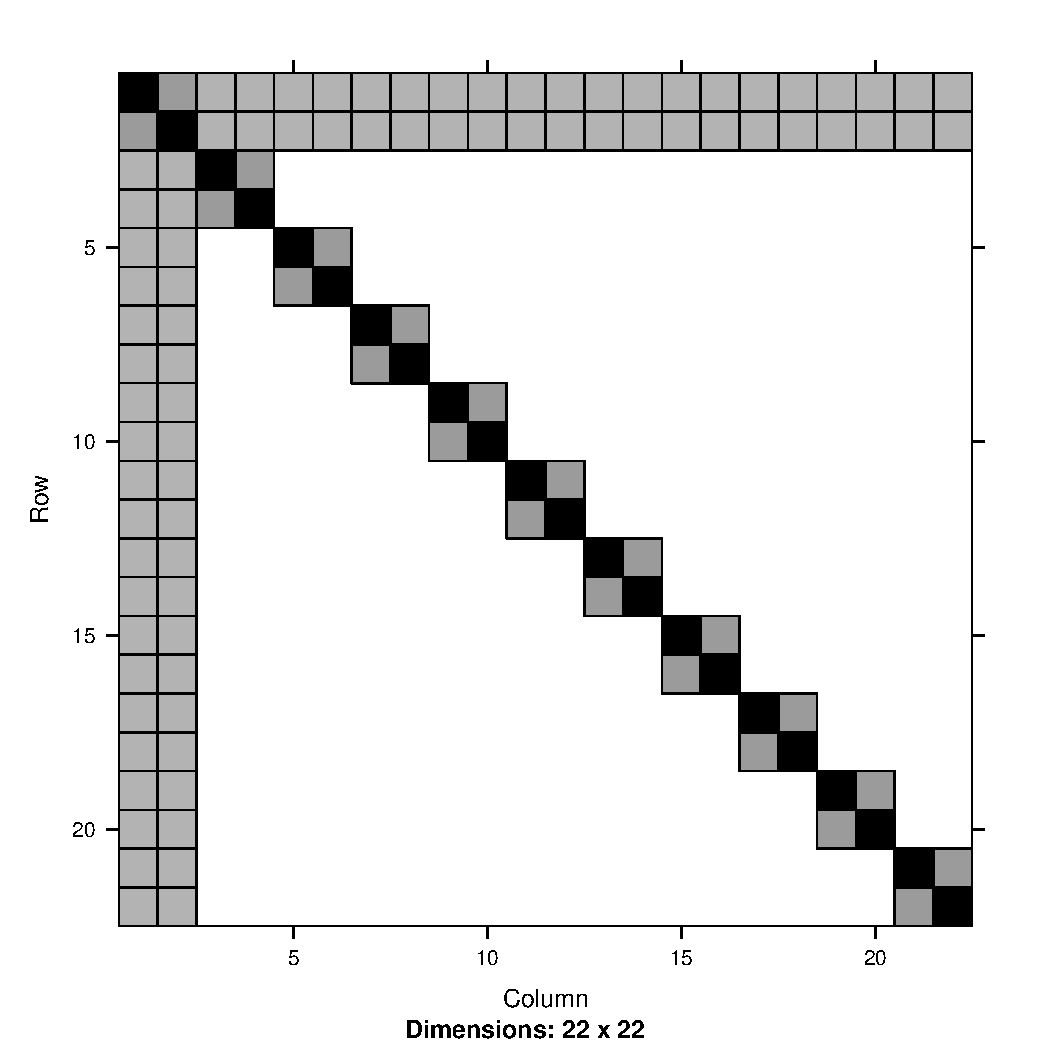
\includegraphics[width=0.35 \textwidth]{mX_mZ_mLambda.pdf}
	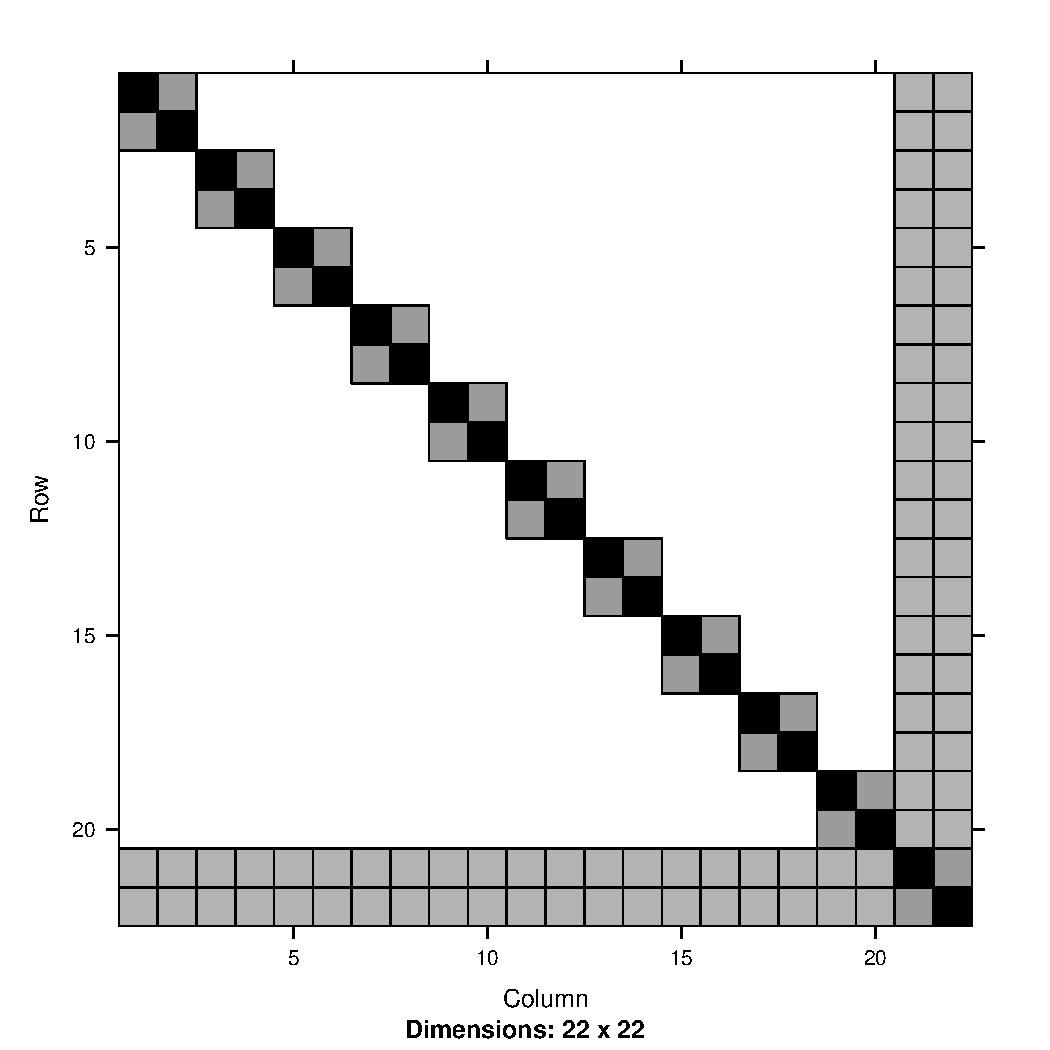
\includegraphics[width=0.35 \textwidth]{mZ_mX_mLambda.pdf}
	\caption{Inverse Covariance matrix of approximate posterior for $\vnu$ -- Fixed effects before random effects
						and random before fixed effects.}
	\label{fig:covfixedrandom}
\end{figure}
	
\begin{figure}[h!]
	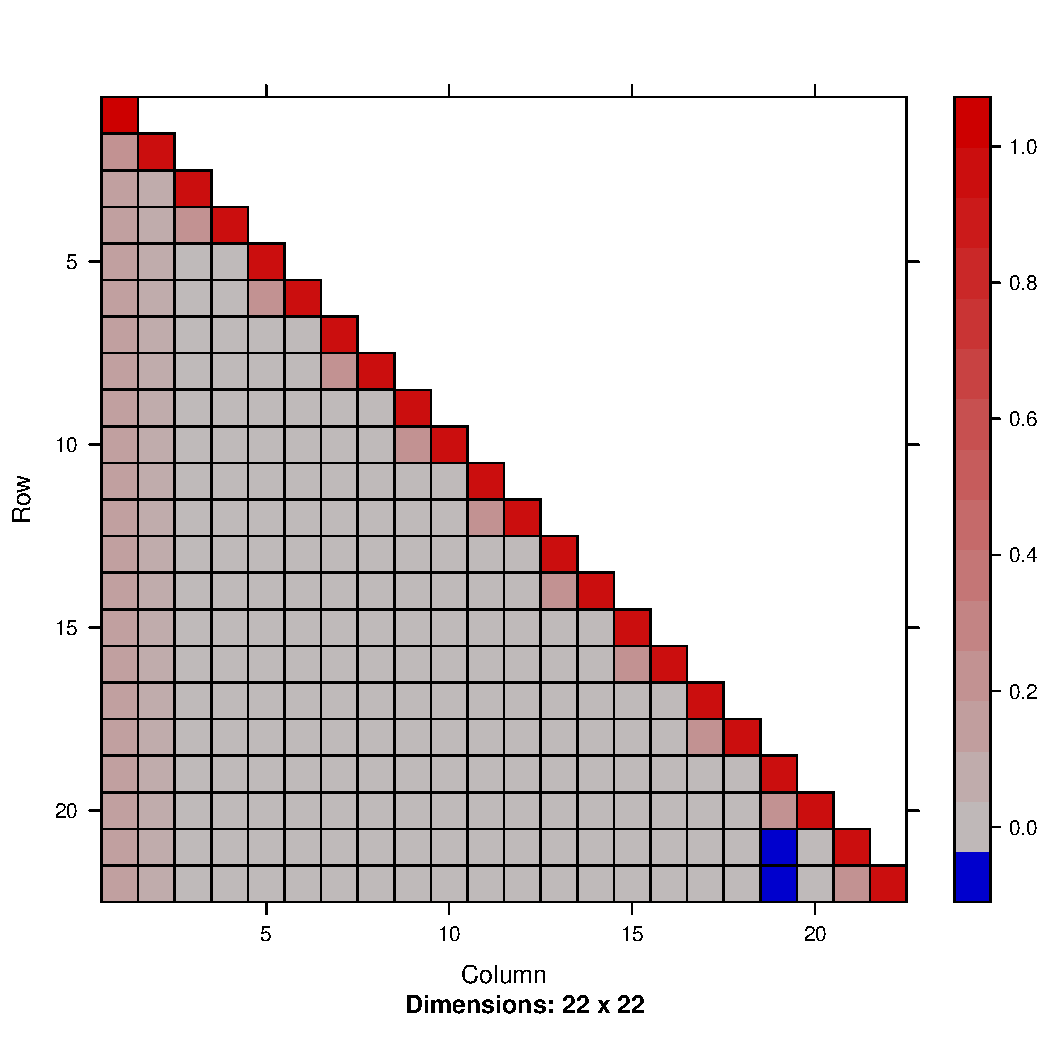
\includegraphics[width=0.35 \textwidth]{mX_mZ_cholesky.pdf}
	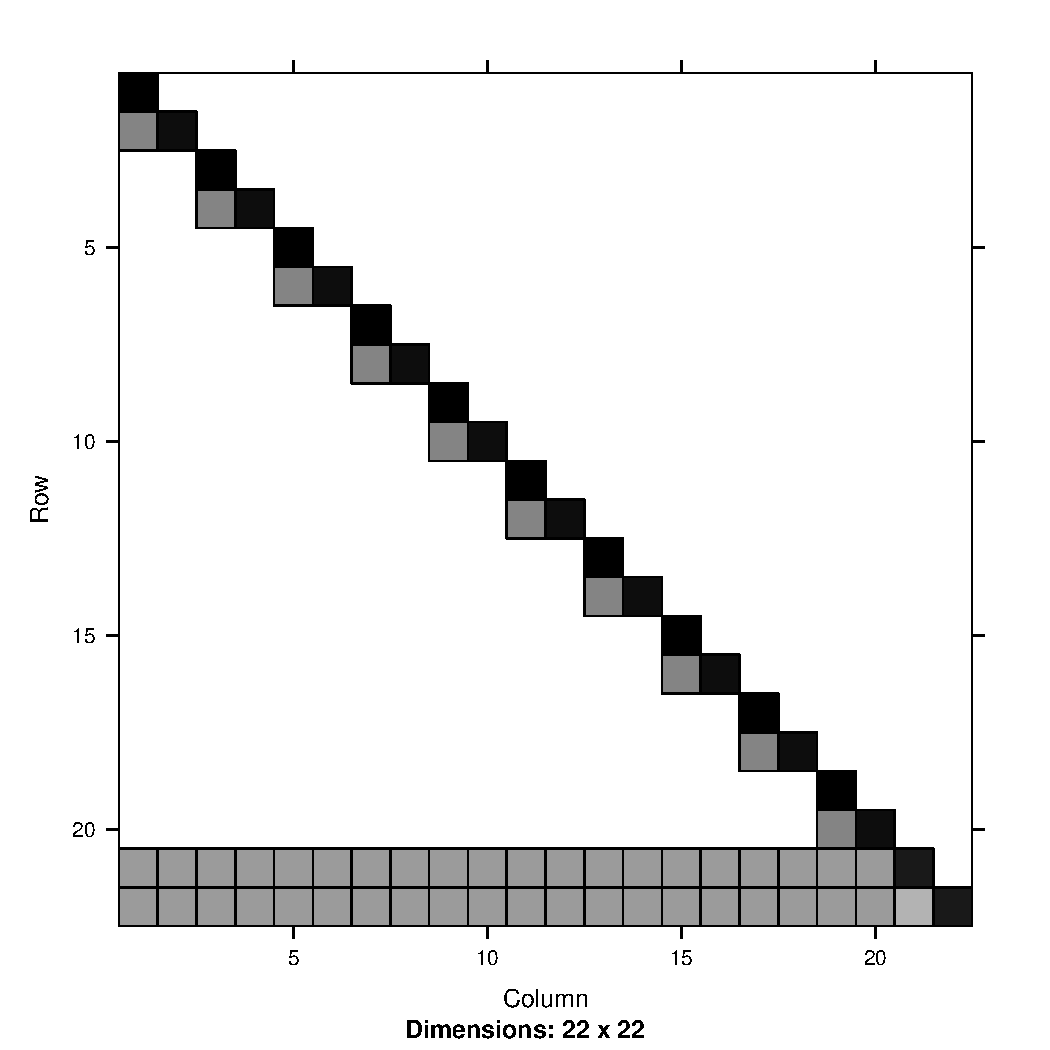
\includegraphics[width=0.35 \textwidth]{mZ_mX_cholesky.pdf}
	\bigskip 
	\caption{Cholesky factor of Inverse Covariance matrix of approximate posterior for $\vnu$ -- Fixed effects 
						before random effects and random before fixed effects.}
	\label{fig:cholfixedrandom}
\end{figure}

\newpage

\subsection{Precision parameterisation}

The GVA is fit by maximising the Gaussian
Variational Lower Bound, which is parameterised by a mean vector $\vmu$ and a
covariance matrix $\mLambda$. The simplest parameterisation of $\vmu$ is the
natural parameterisation, but the covariance matrix has many possible
parameterisations. Covariance matrices are positive semi-definite, and hence
symmetric, so they have a unique Cholesky factorisation. Parameterising the
covariance matrix in terms of the Cholesky factor allows us to represent the
square covariance matrix using only a lower triangular matrix with half as many
non-zero elements. Thus the Cholesky factor is a convenient way to parameterising
covariance matrices.

The variational lower bound of a GVA takes the
form given below.
\begin{equation}
\label{eq:gva_lower_bound_precision_param2}
\begin{array}{ll}
\log \underline{p}(\vy; \vmu, \mLambda) =& \vy^\top \mC \vmu - \vone^\top B(\mC \vmu, \text{diag}(\mC \mLambda \mC^\top)) + \vone^\top c(\vy) \\
&- \tfrac{1}{2} \vmu^\top \mSigma^{-1} \vmu - \tfrac{1}{2} \tr(\mSigma^{-1} \mLambda) \\
&+ \tfrac{1}{2} \log |\mLambda| - \tfrac{1}{2} \log |\mSigma| + \tfrac{d}{2}.
\end{array}
\end{equation}

Let $\mOmega = \mLambda^{-1}$, the precision matrix. Then if we reparameterise
the variational lower bound in terms of $\mOmega$ we obtain the function below.
\begin{equation}
\label{eq:gva_lower_bound_precision_param_omega}
\begin{array}{ll}
F(\mOmega) =& \quad \vy^\top \mC \vmu - \vone^\top B(\mC \vmu, \text{diag}(\mC \mOmega^{-1} \mC^\top)) + \vone^\top c(\vy) \\
&- \tfrac{1}{2} \vmu^\top \mSigma^{-1} \vmu - \tfrac{1}{2} \tr(\mSigma^{-1} \mOmega^{-1}) \\
&- \tfrac{1}{2} \log |\mOmega| - \tfrac{1}{2} \log |\mSigma| + \tfrac{d}{2}.
\end{array}
\end{equation}

When the variational lower bound is optimised, by the first-order optimality
conditions, $\tfrac{\partial F}{\partial \mOmega_{jk}} = \vzero$. Then using
matrix calculus and the properties of the trace operator
\begin{equation*}
\begin{array}{ll}
\tfrac{\partial F}{\partial \mOmega_{jk}} &= -\tfrac{1}{2} \tr(\mOmega^{-1} \tfrac{\partial \mOmega}{\partial \mOmega_{jk}}) + \tfrac{1}{2} \tr(\mSigma^{-1} \mOmega^{-1} \tfrac{\partial \mOmega}{\partial \mOmega_{jk}} \mOmega^{-1}) \\
&\quad -\tfrac{1}{2} \tr\{\mC^\top \text{diag}(B^{(2)}(\mC \vmu, \text{diag}(\mC \mOmega^{-1} \mC^\top))) \mC \mOmega^{-1} \tfrac{\partial \mOmega}{\partial \mOmega_{jk}} \mOmega^{-1}\} \\
&=-\tfrac{1}{2} [ \tr(\mOmega^{-1} \mOmega \mOmega^{-1} \tfrac{\partial \mOmega}{\partial \mOmega_{jk}}) - \tr(\mSigma^{-1} \mOmega^{-1} \tfrac{\partial \mOmega}{\partial \mOmega_{jk}} \mOmega^{-1}) \\
&\quad + \tr\{\mOmega^{-1} \mC^\top \text{diag}(B^{(2)}(\mC \vmu, \text{diag}(\mC \mOmega^{-1} \mC^\top))) \mC \mOmega^{-1} \tfrac{\partial \mOmega}{\partial \mOmega_{jk}}\} ] \\
&= -\tfrac{1}{2} \tr\{\mOmega^{-1}[\mOmega - \mC^\top \text{diag}(B^{(2)}(\mC \vmu, \text{diag}(\mC \mOmega^{-1} \mC^\top))) \mC - \mSigma^{-1} ] \mOmega^{-1} \tfrac{\partial \mOmega}{\partial \mOmega_{jk}}\}
\end{array}
\end{equation*}

As $\mOmega^{-1} \ne \vzero$ and $\tfrac{\partial \mOmega}{\partial
\mOmega_{jk}} \ne \vzero$, this implies $\mOmega = \mC^\top
\text{diag}(B^{(2)}) \mC + \mSigma^{-1}$. Thus the sparsity of $\mOmega$
depends on the structure of $\mC$ and $\mSigma$, which depends on the model
specified.

We optimise over the space $(\vmu, \overline{\mR})$ as in the Section
\ref{sec:param}, but now the elements of the Cholesky factor are parameterised
as
\begin{equation*}
\label{eq:cholesky_element_precision_param}
	\mR_{ij} =
	\begin{cases}
		\exp(-\overline{\mR}_{ij}), & i = j             \\
		\overline{\mR}_{ij},        & i > j             \\
		0,                          & \text{otherwise}.
	\end{cases}
\end{equation*}
	
\noindent This new choice of parameterisation allows us to calculate
$\frac{1}{2} \text{diag}(\mC \mLambda \mC^\top)$ by solving the linear systems
$\mR \va = \mC_{i}, i=1, \ldots, n$ for   $\va$ and then calculating
$\va^\top\va$ where $\mC_{i} = $ the $i$th row of $\mC$, rather than
calculating $\text{diag}(\mC \mLambda \mC^\top)$ directly.
	
Another advantage of parameterising using the precision matrix is that
the covariance matrix contains the marginal covariances between the elements of
$\vnu$, while the precision matrix contains the conditional covariances
between those elements. In generalised linear mixed models, fixed and random
effects are conditionally independent, implying sparsity in the precision
matrix although not necessarily in the covariance matrix.

A final advantage of this parameterisation is its' greater numerical accuracy.
Matrix multiplication and back substitution are both equally numerically
accurate and stable - as shown in \cite{Golub:1996:MC:248979} \S2.7.8 and
\S3.1.2 or \cite{trefethen97} Lecture 17, and the precision matrix will be
sparse due to the specification of the mixed model/conditional independence.
This implies that the numerical accuracy of the inversion will be higher as
there are fewer non-zero entries in the Cholesky factor of the precision matrix
than of the Cholesky factor of the covariance matrix. Thus parameterising the
variational lower bound in terms of the precision matrix will have the same or
higher numerical accuracy than parameterising in terms of the covariance
matrix.

\section{Numerical results}
\label{sec:results}
The accuracy of each of the model fitting algorithms presented in Section
\ref{sec:gaussian} was assessed by comparing the approximating distribution of
each parameter with the posterior distribution of MCMC
samples of that parameter. One million MCMC samples were
generated using \texttt{RStan} \citep{Carpenter2016, StanDevelopmentTeam2016}.
The accuracy of examples using random intercept, random slope and spline models
were evaluated using this method.

\newpage 
		
\subsection{Simulated data}
For each of these simulations, the model is as presented in Section
\ref{sec:model}. Several common application scenarios were simulated and their
accuracy evaluated. A random intercept model was simulated with $\vbeta = (2,
1)^\top$, $\rho = 0.5$, $m = 20$, $n_i = 10$ and $b = 1$. The results are
presented in Table \ref{tab:accuracy_int}. A random slope model was simulated
with $\vbeta = (2, 1)^\top$, $\rho = 0.5$, $m = 20$, $n_i = 10$ and $b = 2$.
The results are presented in Table \ref{tab:accuracy_slope}. Spline model was
fit to a data set generated from the function $3 + 3 \sin{(\pi x)}$ on the
interval $[-1, 1]$. The resulting model fits are presented in Figure
\ref{fig:spline}.
		
To assess the speed of each approach, a test case was constructed of a random
slope model with $m=50$ groups, each containing $n_i = 100$ individuals. A
model was then fit to this data set ten times using each algorithm, and the
results averaged. These results are presented in Table
\ref{tab:application_slope_speed}.

\begin{table}
{\footnotesize 
	\begin{tabular}{|l|rr|}
		\hline
		Algorithm & Mean (seconds) & Standard deviation (seconds) \\
		\hline
		Laplace's method & $0.37$ & $0.07$ \\
		GVA covariance parameterisation & $2.04$ & $1.24$ \\
		% Why is this slower?
		GVA precision parameterisation & $0.38$ & $0.66$ \\
		GVA fixed point & $0.05$ & $0.07$ \\
		\hline
	\end{tabular}
}\bigskip
	\caption{Table of results - Speed.}
	\label{tab:application_slope_speed}
\end{table}

% The stability of the algorithms was confirmed by running them on 10,000
% different data sets that were randomly generated after having initialised the
% random number generator with different seeds.
		
The median accuracy of the algorithms was assessed by running them on 100
randomly generated data sets. The	results are presented in Figure
\ref{fig:median_accuracy_intercept} and Figure \ref{fig:median_accuracy_slope}.
		
% Figure: Median accuracy graph intercept
\begin{figure}[h]
	\begin{center}
		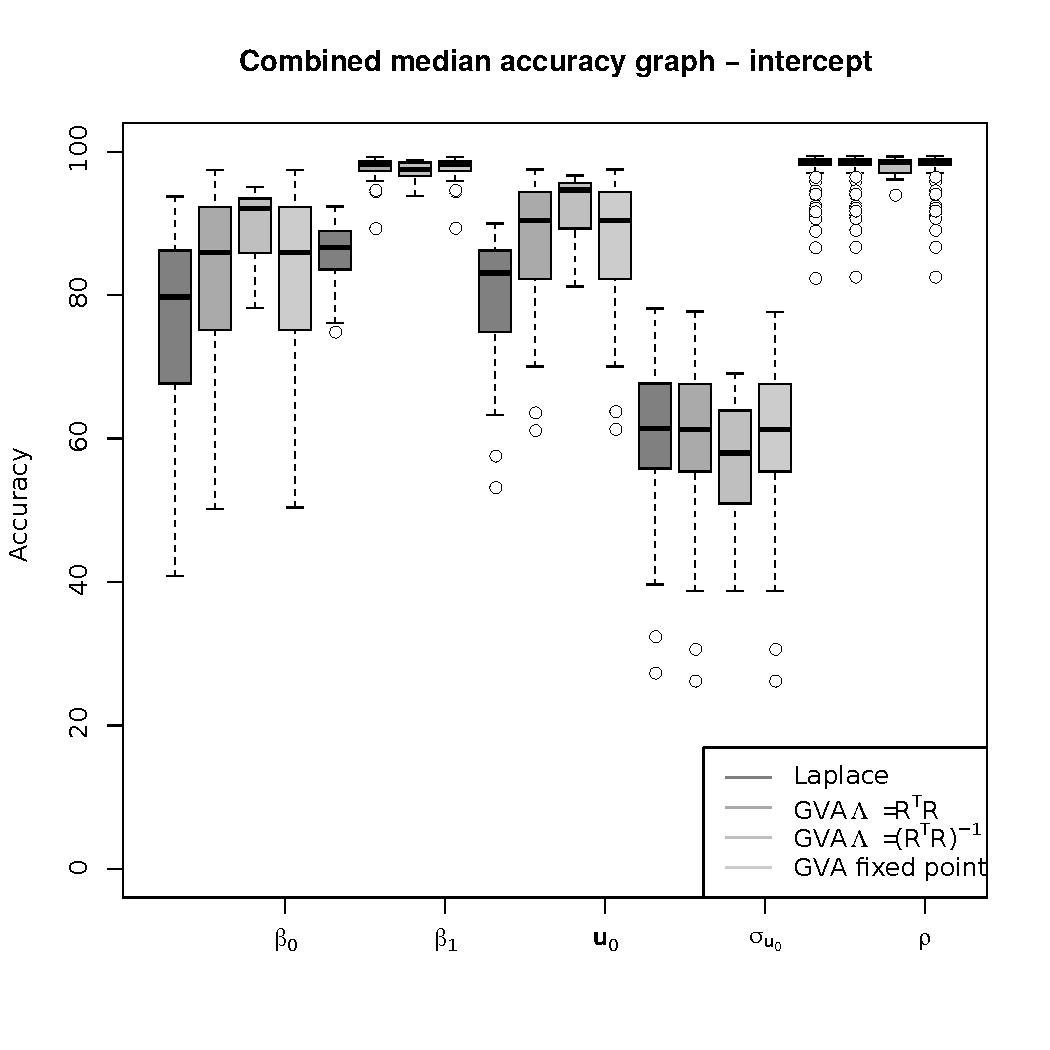
\includegraphics[width=0.99\textwidth]{code/results/median_accuracy_combined_intercept.pdf}
		\bigskip
		\caption{Boxplots of accuracies of the parameter estimates for a random intercept model after 100 repeated
							runs on simulated data. We see that the accuracy of the parameter estimates is quite stable,
							and the median accuracies are high.}
		\label{fig:median_accuracy_intercept}
	\end{center}
\end{figure}
		
% Figure: Median accuracy graph slope
\begin{figure}[h]
	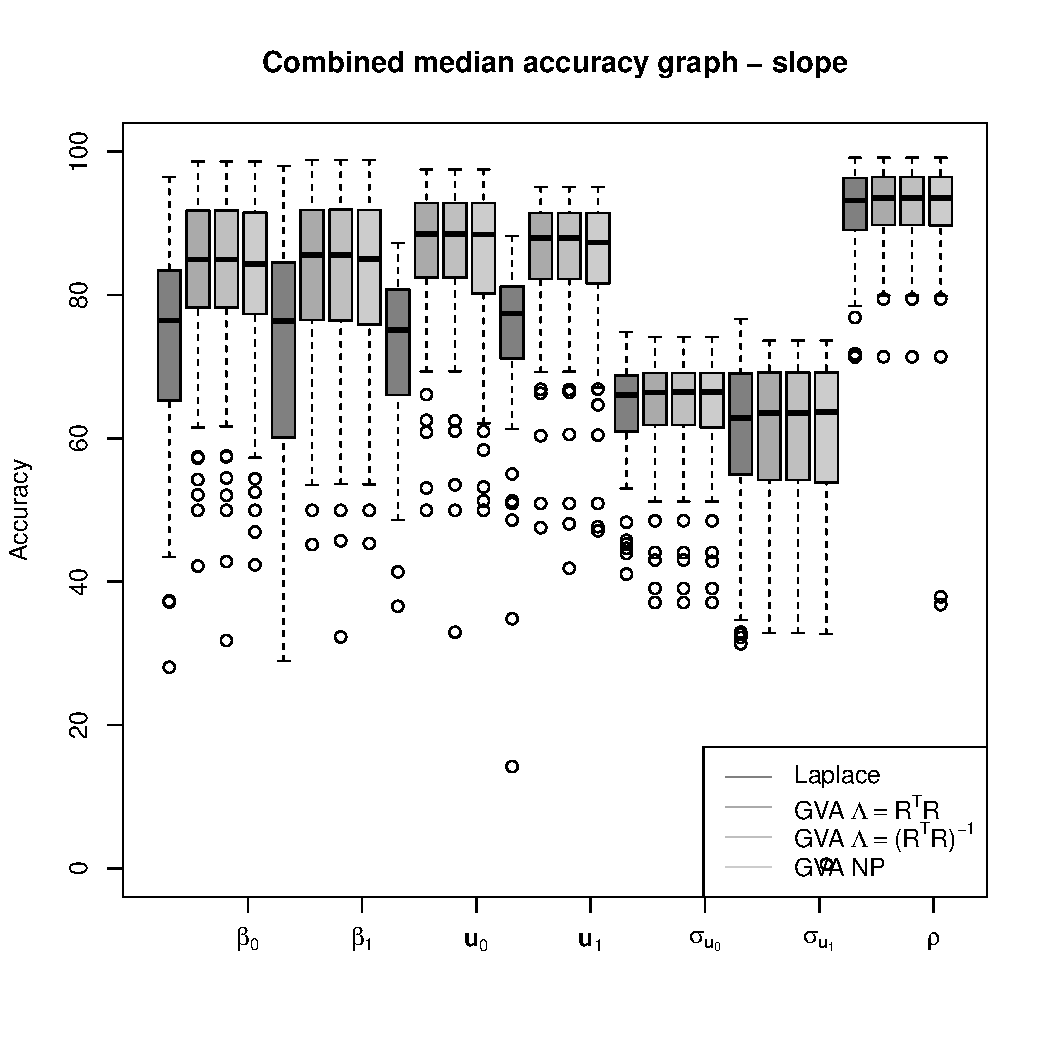
\includegraphics[width=\textwidth]{code/results/median_accuracy_combined_slope.pdf}\bigskip 
	\caption{Boxplots of accuracies of the parameter estimates for a random slope model after 100 repeated
							runs on simulated data. We see that the accuracy of the parameter estimates is quite stable,
							and the median accuracies are high.}
	\label{fig:median_accuracy_slope}
\end{figure}
		
% Table of accuracy results - intercept model
\begin{table}
{\footnotesize
	\begin{tabular}{|l|rrrr|}
		\hline
		                   & Laplace's Method & GVA $(\mLambda = \mR \mR^\top)$ & GVA NP $(\mLambda = (\mR \mR^\top)^{-1})$ & GVA FP \\
		\hline
		$\vbeta_1$         & $85\%$           & $90\%$                          & $91\%$                                    & $90\%$ \\ 
		$\vbeta_2$         & $76\%$           & $98\%$                          & $99\%$                                    & $99\%$ \\ 
		Mean of $\vu$'s      & $81\%$           & $94\%$                          & $94\%$                                    & $94\%$ \\
		$\sigma^2_{\vu_1}$ & $66\%$           & $66\%$                          & $66\%$                                    & $66\%$ \\ 
		$\rho$             & $99\%$           & $99\%$                          & $99\%$                                    & $99\%$ \\ 
		\hline
	\end{tabular}
}\bigskip
	\caption{Table of accuracy - Random intercept model.}
	\label{tab:accuracy_int}
\end{table}
		
\begin{table}
	{\footnotesize
	\begin{tabular}{|l|rrrr|}
		\hline
		                   & Laplace's Method & GVA $(\mLambda = \mR \mR^\top)$ & GVA $(\mLambda = (\mR \mR^\top)^{-1})$ & GVA FP \\
		\hline
		$\vbeta_1$         & $67\%$             & $88\%$                            & $88\%$                                   & $88\%$   \\
		$\vbeta_2$         & $70\%$             & $89\%$                            & $88\%$                                   & $89\%$   \\
		Mean of $\vu$      & $70\%$             & $91\%$                            & $91\%$                                   & $91\%$   \\
		$\sigma^2_{\vu_1}$ & $71\%$             & $73\%$                            & $73\%$                                   & $73\%$   \\
		$\sigma^2_{\vu_2}$ & $68\%$             & $69\%$                            & $69\%$                                   & $69\%$   \\
		$\rho$             & $91\%$             & $90\%$                            & $90\%$                                   & $90\%$   \\
		\hline
	\end{tabular}
}\bigskip
	\caption{Table of accuracy - Random slope model.}
	\label{tab:accuracy_slope}
\end{table}
		
% \begin{table}
% \caption{Table of accuracy - Splines}
% \label{tab:accuracy_spline}
% \begin{tabular}{|l|l|}
% \hline
% Approximation & Accuracy \\
% \hline
% Laplace's Method & 0.969 \\
% GVA & 0.969 \\
% GVA NP & 0.969 \\
% GVA NR & 0.969 \\
% \hline
% \end{tabular}
% \end{table}
		
\begin{figure}[h]

	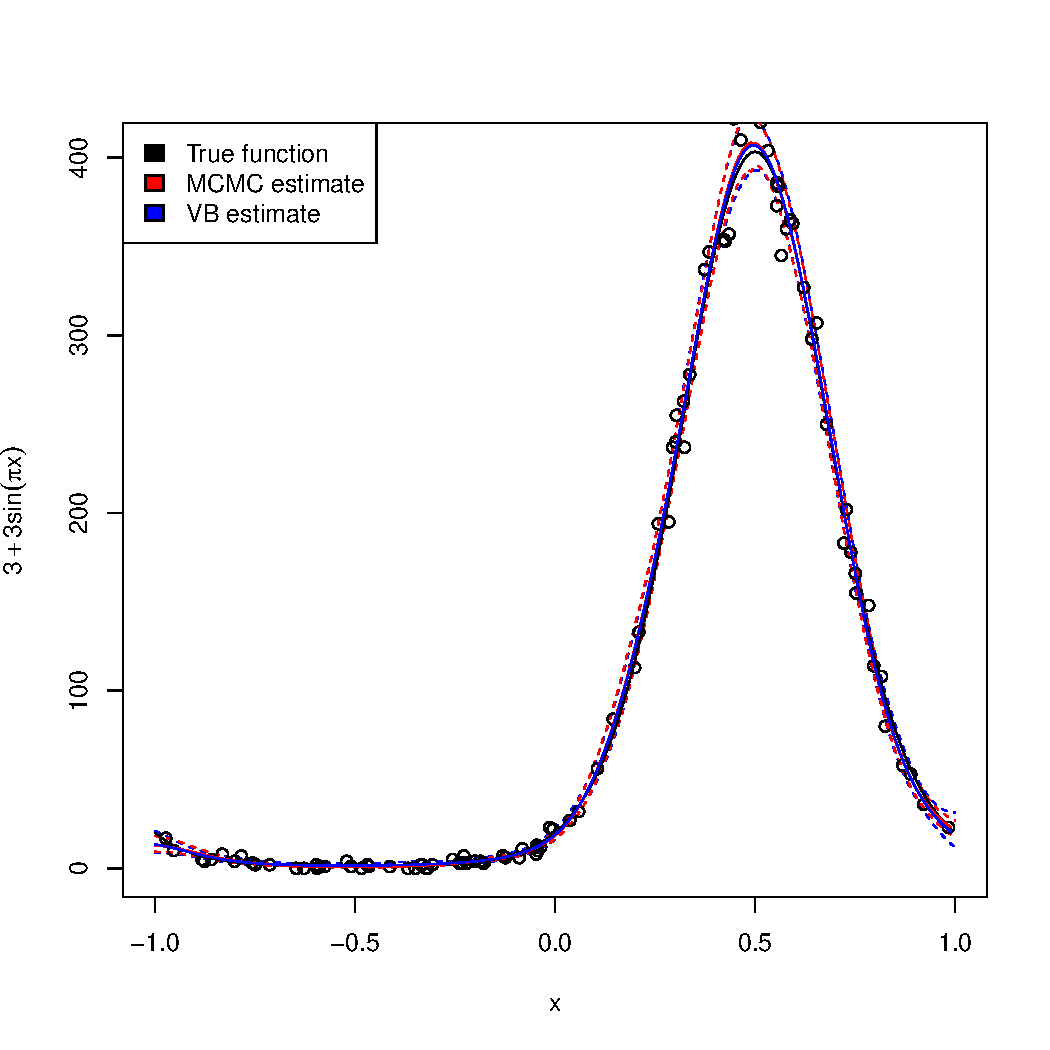
\includegraphics[width=  0.9\textwidth]{code/results/accuracy_plots_spline_gva2.pdf}
	
	\label{fig:spline}  
\caption{Comparison of VB and MCMC spline fits with the true function.}	
\end{figure}

  
		
\subsection{Numerical stability of the parameterisation}

The stability of this scheme was tested by calculating the accuracy of the
approximations fit with a range of safe exponential thresholds, the results of
which are presented in Figure \ref{fig:stability_accuracy}. The variational
approximation was found to be stable, with the accuracy largely insensitive to
the choice of threshold.

\begin{figure}[h]
	\includegraphics[width=0.95 \textwidth]{code/stability_intercept.pdf}
	\label{fig:stability_accuracy}
	\caption{Accuracy of approximation of parameters versus the safe exponential threshold.}
\end{figure}

We repeated our numerical experiments with the new parameterisation, varying
the threshold within reasonable bounds and found that the numerical experiments
no longer resulted in overflow, and that the numerical accuracy of the
approximation was still very good.

The stability of the GVA algorithm with the parameterisation $\mLambda =
(\mR^\top \mR)^{-1}$ depends on the threshold chosen for the safe exponential
function. When the threshold is set to $2$, the algorithm is stable for all
starting points within the grid except $6$. When the threshold is set to
$\infty$, equivalent to using the naive $\exp$ parameterisation, the algorithm
encounters numerical errors for every starting point on the  grid.

\newpage 
	
\subsection{Stability of the GVA precision parameterisation algorithm for different starting points}
The numerical stability of each fitting algorithm in Section \ref{sec:gaussian}
was assessed by initialising each algorithm from a range of different starting
points. Errors due to numerical instability and the fitted $\vmu$ were recorded
for each starting point.
		
A data set of 100 individuals in ten groups ($m=10$) was generated from a model
with a fixed intercept and slope, and a random intercept. $\vmu$ was
initialised from a grid of points on the interval $[-4.5, 5]$ for intercept and
slope, spaced $0.1$ apart. The error counts are presented in Table
\ref{tab:stability_results}. Plots of the starting locations which resulted in
numerical errors when the fitting algorithm was run are presented in
\ref{fig:stability_locations_gva}.
		
\begin{table}
	\begin{tabular}{|l|r|}
		\hline
		Algorithm                            & Error count \\
		\hline
		Laplace's algorithm                  & $12$          \\
		GVA $\mLambda = \mR^\top \mR$        & $1306$       \\
		GVA $\mLambda = (\mR^\top \mR)^{-1}$ & $6$           \\
		GVA NR fixed point                   & $992$         \\
		\hline
	\end{tabular}\bigskip
	\caption{Count of numerical errors for each algorithm during stability tests.}
	\label{tab:stability_results}
\end{table}

The GVA algorithm with the $\mLambda = (\mR \mR^\top)^{-1}$ parameterisation
was less prone to instability due to starting point when the safe exponential
parameterisation was used then when it was not used, as can be seen from Figure
\ref{fig:stability_locations_gva}. % FIXME: Add error counts
% TODO: I hate this graph. Re-do it.
\begin{figure}[h]
	\includegraphics[width=0.45 \textwidth]{code/safe_exp_stability.pdf}
	\includegraphics[width=0.45 \textwidth]{code/no_safe_exp_stability.pdf}
	\label{fig:stability_locations_gva}\bigskip
	\caption{
        Starting locations which caused the GVA fitting algorithm to fail with
        numeric errors. The true model had fixed parameters $\vbeta = (2,
        1)^\top$ and random intercepts. There were ten groups in the
        hierarchical model each	with ten individuals $(m=10, n_i=10)$. In the
        left figure the starting points which lead to numeric errors when the
        safe exponential was used are shown, while in the right figure the
        starting points which lead to numeric errors when the safe exponential
        was not used are plotted.
    }
\end{figure}

\subsection{Stability of the GVA fixed point algorithm for different starting
points}
The naive fixed point algorithm was extremely unstable for many starting
points, as can be seen from Figure \ref{fig:stability_locations_nr}.  The
variant of the algorithm which checked whether the inversion of the
$\mLambda_{\vu \vu}$ block of $\mLambda$ was performed successfully was much
more stable, and did not suffer from any numeric errors at all over the range
of starting points we tested.  The algorithm is able to abort safely, and allow
the Variational Bayes algorithm to update the other parameters before trying to
fit the Gaussian component of the model again until the correct parameters are
accurately estimated.

% Generated by Rscript code/plot_local_solutions.R -i code/local_solutions_gva_nr_error_locations_no_protections.csv -o code/local_solutions_gva_nr_error_locations_no_protections.pdf
\begin{figure}[h!]
	\includegraphics[width=0.99 \textwidth]{code/local_solutions_gva_nr_error_locations_no_protections.pdf}
	\label{fig:stability_locations_nr} \bigskip 
    \caption{Starting locations which caused the fixed point fitting algorithm to fail with numeric errors. The true model had fixed parameters $\vbeta = (2, 1)^\top$ and random intercepts. There were ten groups in the
	hierarchical model each	with ten individuals $(m=10, n_i=10)$.}
\end{figure}

\section{Applications}
We now present numerical results for the application of our model fitting
algorithms to several publicly available data sets.

\label{sec:application}

\subsection{Poisson example without zero-inflated component -- Police stops}
\label{sec:police_stops}
The data set used for this example was the police stop example from Chapter 15
of \cite{Gelman2007}.  The model fit was
\begin{equation*}
	\vy_{ep}        \sim \text{Poisson}(n_{ep} e^\vnu)
\end{equation*}
\noindent where $\vnu = {\beta_0 + \beta_e \text{ethnicity}_e + \alpha_{c} \text{crime} + \vu_p}$, 
with priors
$$
\valpha \sim \N(0, \sigma_\valpha^2), 
\qquad 	
\vbeta \sim \N(0, \sigma_\vbeta^2), \quad \mbox{ and } \quad 
	\vu_p \sim \N(0, \sigma_\vu^2),
$$

\noindent the index
$p$ corresponds to each precinct, $e$ is the index of ethnicity
(African-Americans, hispanics or whites), and $c$ is the index of category of
crime (violent crimes, weapons crimes, property crimes or drug crimes). The
random intercepts $u_p$ allow for variation in the base rates of stops across
precincts, the coefficients $\beta_j$ measure the effect of ethnicity on the
rate of police stops and the coefficients $\alpha_k$ measure the effect of
each type of crime on the rate. The model finds the relationship between the
number of police stops in each precinct and  ethnicity for each type of crime.

The model was fit using the GVA algorithm with the $\mLambda = (\mR^\top
\mR)^{-1}$ parameterisation, using the prior $a_\rho = 3$, $b_\rho = 1$ on
$\rho$. Accuracy of the approximation was assessed by comparing the fitted
distribution for each parameter to a kernel density estimate of the parameter's
distribution from 1 million samples from the equivalent model using
Stan. The results are presented in Table \ref{tab:application_police_stops} and
Figure \ref{fig:police_stops}.

\begin{figure}
\centering
  \includegraphics[page=1,scale=0.45]{code/results/accuracy_plots_application2_GVA.pdf}
  \includegraphics[page=2,scale=0.45]{code/results/accuracy_plots_application2_GVA.pdf}
  \includegraphics[page=3,scale=0.45]{code/results/accuracy_plots_application2_GVA.pdf}
  \includegraphics[page=7,scale=0.45]{code/results/accuracy_plots_application2_GVA.pdf}
  \includegraphics[page=81,scale=0.45]{code/results/accuracy_plots_application2_GVA.pdf}
  \includegraphics[page=82,scale=0.45]{code/results/accuracy_plots_application2_GVA.pdf}
\caption{Accuracy of parameter estimates for police stops.}
\label{fig:police_stops}
\end{figure}

% Table of results
\begin{table}
	{\footnotesize 
	\begin{tabular}{|l|rrrr|}
		\hline
		Covariate                     & Posterior Mean & Lower 95\% CI & Upper 95\% CI & Accuracy \\
		\hline
		Intercept [African-Americans] & $4.04$          & $3.98$           & $4.07$          & 85\%   \\
		$\beta_2$ [hispanics]         & $-0.45$         & $-0.46$          & $-0.43$         & 99\%   \\
		$\beta_3$ [whites]            & $-1.38$         & $-1.40$          & $-1.37$         & 99\%   \\
		$\alpha_1$ [weapons crimes]   & $0.58$          & $0.57$           & $0.59$          & 90\%   \\
		$\alpha_2$ [property crimes]  & $-0.19$         & $-0.21$          & $-0.17$         & 92\%   \\
		$\alpha_3$ [drug crimes]      & $-0.75$        & $-0.77$          & $-0.73$         & 95\%   \\
		Random intercept              & $1.32$         & $-0.19$         & $2.20$         & 87\%   \\
		$\sigma^2_{\vu}$              & $8.57$          & $1.02$           & $24.35$         & 67\%     \\
		\hline
	\end{tabular}
}\bigskip
	\caption{Table of results - Police stops.}
	\label{tab:application_police_stops}
\end{table}

% Table of speeds
\begin{table}
	\begin{tabular}{|l|r|}
		\hline
		Algorithm & Time  in seconds \\
		\hline
		Laplace & $0.07$ \\
		%GVA covariance parameterisation & $6.02$ \\ % TODO: Did not run
		GVA precision paramaterisation & $0.90$ \\
		GVA fixed point & $0.06$ \\
		\hline
	\end{tabular}\bigskip
	\caption{Table of speeds - Police stops.}
	\label{tab:police_stop_speeds}
\end{table}

\subsection{Zero--inflated example -- Cockroaches in apartments}
\label{sec:cockroaches}

The model described in this section was fit  to the cockroach data set from
Section 6.7 of \cite{Gelman2007}, taken from a study on the effect of
integrated pest management in controlling cockroach levels in urban apartments.
The data set contains data on 160 treatment and 104 control apartments, along
with the response $y_i$ in each apartment of the number of cockroaches caught
in a set of traps. The apartments had the traps deployed for different numbers
of days, referred to as trap days, which was handled by using a log offset
\citep{Agresti2002}. The predictors in the data set included the pre-treatment
roach level, a treatment indicator, the time of the observation and an
indicator for whether the apartment is in a senior building restricted to the
elderly.
		
In the example application presented in this paper, the zero component
represents an apartment completely free of roaches, while the non-zero
component represents an apartment where roaches have been able to live and
reproduce, possibly in spite of pest control treatment aimed at preventing them
from doing so. The model fit was
\begin{equation*}
    y_i = \begin{cases}
        0, &\text{ if } R_i = 0, \text{ and } \\
        \text{Poisson}(e^{\mX_i \vbeta + \mZ_i \vu}), & \text{ if } R_i = 1,
	\end{cases}
\end{equation*}
with priors 
$$
\begin{array}{c} 
R_i \sim \text{Bernoulli}(\rho), 
\quad 
\rho \sim \text{Beta}(a, b),
\quad \vbeta \sim \text{N}(\vzero, \sigma^2_{\vbeta} \mI), 
\\
\quad \vu \sim
\text{N}(\vzero, \mSigma) \quad \text{ and } \quad \mSigma \sim
\text{Inverse-Wishart}(\mPsi, v)
\end{array} 
$$

\noindent and prior hyperparameters $a = 1$, $b = 1$,
$\sigma^2_\vbeta = 10^5$, $\mPsi = 10^{-5} \mI$ and $v = 2$.  These priors were
chosen to be vaguely informative for the variance components and a uniform
prior for the zero-inflation proportion latent variable $\rho$. The fixed
effects covariates included in the model were time in days and time in days
$\times$ pest control treatment. A random intercept to account for variation
between the apartment buildings was included.
		
The GVA algorithm with the $\mLambda = (\mR^\top \mR)^{-1}$ parameterisation
was used to fit a random intercept model to the Roaches data set provided in
\cite{Gelman2007}. The fitted coefficients and accuracy results are presented
in Table \ref{tab:application_roaches}.
		
%       lci  uci
% 1  3.179 3.157 3.201
% 2 -0.046 -0.053 -0.039
% 3 -0.420 -0.434 -0.406
% 1 -0.976 -1.015 -0.936
% 2 -0.309 -0.323 -0.295
% 3 -0.947 -0.963 -0.930
% 4 -2.129 -2.384 -1.874
% 5 -3.230 -3.490 -2.970
% 6 -3.099 -3.404 -2.794
% 7 -1.290 -1.326 -1.255
% 8 -0.956 -0.991 -0.921
% 9 -2.404 -2.600 -2.209
% 10 -1.076 -1.123 -1.029
% 11 -1.079 -1.107 -1.052
% 12 -1.681 -1.737 -1.624
		
%> round(cbind(fit1$vmu, lci, uci), 3)
% fit1$a_rho
% [1] 377.2375
% > fit1$b_rho
% [1] 152.7625
		
\begin{table}
	{\footnotesize
	\begin{tabular}{|l|rrrr|}
		\hline
		Covariate          & Posterior Mean & Lower 95\% CI & Upper 95\% CI & Accuracy \\
		\hline
		Intercept          & $3.42$						& $3.20$ 					& $3.65$          & $96\%$     \\
		Time               & $-0.14$        & $-0.05$       & $-0.02$       & $98\%$     \\
		Time:Treatment     & $-0.31$        & $-0.43$       & $-0.14$       & $99\%$     \\
		Random intercept   & $-1.60$        & $-1.71$       & $-1.49$       & $98\%$     \\
		$\sigma^2_{\vu_1}$ & $3.29$           & $2.02$          & $8.48$          & $64\%$     \\
		$\rho$             & $0.51$           & $0.50$          & $0.55$          & $63\%$     \\
		\hline
	\end{tabular}
}
\bigskip
	\caption{The posterior means, 95\% credible intervals and accuracy of the fixed and random
						effects, $\sigma_{\vu_1}^2$ and $\rho$ for the Roach model.}
	\label{tab:application_roaches}
\end{table}

\begin{table}
	{\footnotesize
	\begin{tabular}{|lr|}
	\hline
	Algorithm & Time in seconds \\
	\hline
	Laplace & $0.68$ \\
	GVA & $2.02$ \\
	GVA inv. param & $1.70$ \\
	GVA fixed point & $0.17$ \\
	\hline
	\end{tabular}
}
	\label{tab:application_roaches_runtime}\bigskip
	\caption{The runtimes in seconds for fitting algorithms when fitting the roach model.}
\end{table}
		
\begin{figure}[h]
	\centering
	%\includepdf[width=75mm,height=75mm,pages={1,2,3,16},nup=2x2]{code/results/accuracy_plots_application_GVA2.pdf}
	\includegraphics[page=1,scale=0.35]{code/results/accuracy_plots_application_GVA_inv_param.pdf}
	\includegraphics[page=2,scale=0.35]{code/results/accuracy_plots_application_GVA_inv_param.pdf}
	\includegraphics[page=3,scale=0.35]{code/results/accuracy_plots_application_GVA_inv_param.pdf}
	\includegraphics[page=4,scale=0.35]{code/results/accuracy_plots_application_GVA_inv_param.pdf}
	\includegraphics[page=16,scale=0.35]{code/results/accuracy_plots_application_GVA_inv_param.pdf}
	\includegraphics[page=17,scale=0.35]{code/results/accuracy_plots_application_GVA_inv_param.pdf}
	\caption{Accuracy graphs for roach model.}
	\label{fig:accuracy_roach}
\end{figure}
		
\subsection{Example - Biochemists}
\label{sec:biochemists}

The model described in this section was fit to the biochemistry data set
analysed by \cite{Long1990}. The sample was taken from 915 biochemistry
graduate students. The outcome $\vy_i$ is the number of articles published in
the last three years of the PhD. The covariates were the gender of the student,
coded $1$ for female and $0$ for male, the marital status of the student ($1$
for married, $0$ for unmarried), the number of children under age six and the
prestige of the PhD program.

In this example application, the zero component represents the number of
biochemists who did not publish any articles during the last three years of
their PhD. Examination of the data reveals that this number is higher than
would be expected if the data followed a purely Poisson distribution -- 30\% of
biochemistry graduate students published no articles in their final years
whereas a Poisson distribution would predict only 18\%. This justifies our
choice of model. The model fit was
$$
	y_i = \begin{cases}
	\begin{array}{ll}
	0, & \text{if} R_i = 0, \text{ and }\\
	\text{Poisson}(e^\vnu), & \text{if} \phantom{-} R_i = 1,
	\end{array}
	\end{cases}
$$

\noindent where $\vnu = \vbeta_1 + \vbeta_2 \text{female} + \vbeta_3
\text{married} + \vbeta_4 \text{children under age 6} + \vbeta_5 \text{PhD}$,
with priors
$R_i \sim \text{Bernoulli}(\rho), 
\rho \sim \text{Beta}(A, B) \text{ and } 
\vbeta \sim \text{N}(0, \sigma_{\vbeta}^2 \mI)$
and $A=1$, $B=1$ and $\sigma_\vbeta^2 = 10,000$. The model was fit
using the GVA precision parameterisation algorithm. The resulting model fit is
presented in Table \ref{tab:biochemists_results} The accuracy of the parameter
estimates is presented in Figure \ref{fig:biochemists}. As this is a fixed
effects model with a large number of samples relative to the number of
parameters being fit, we are able to estimate all of the parameters with great
accuracy.

% This diagram looks a bit dodgy. It's correct, but the titles are missing
% from the edges. Perhaps you should regenerate it.
\begin{figure}[h]
\centering
 % \includegraphics{code/results/accuracy_plots_application_biochemists_GVA_inv_param-nup.pdf}
	\includegraphics[page=1,scale=0.35]{code/results/accuracy_plots_application_biochemists_GVA_inv_param.pdf}
	\includegraphics[page=2,scale=0.35]{code/results/accuracy_plots_application_biochemists_GVA_inv_param.pdf}
	\includegraphics[page=3,scale=0.35]{code/results/accuracy_plots_application_biochemists_GVA_inv_param.pdf}
	\includegraphics[page=4,scale=0.35]{code/results/accuracy_plots_application_biochemists_GVA_inv_param.pdf}
	\includegraphics[page=5,scale=0.35]{code/results/accuracy_plots_application_biochemists_GVA_inv_param.pdf}
	\includegraphics[page=6,scale=0.35]{code/results/accuracy_plots_application_biochemists_GVA_inv_param.pdf}
\label{fig:biochemists}
\caption{Accuracy of the approximations of the parameters fit to the biochemists data.}
\end{figure}

\begin{table}
	{\footnotesize 
	\begin{tabular}{|l|rrrr|}
		\hline
		Covariate          & Posterior Mean & Lower 95\% CI & Upper 95\% CI & Accuracy \\
		\hline
		Intercept & $0.86$ & $0.65$ & $1.06$ &  $95\%$ \\
		Female & $-0.18$ & $-0.29$ & $-0.08$ &  $95\%$ \\
		Married & $0.06$ & $-0.05$ & $0.18$ & $96\%$ \\
		Children under age 6 & $-0.08$ & $-0.15$ & $-0.01$ & $97\%$ \\
		PhD & $0.03$ & $-0.02$ & $-0.01$ & $97\%$ \\
		\hline
	\end{tabular}
}			
	\label{tab:biochemists_results}\bigskip
	\caption{The posterior means, 95\% credible intervals and accuracy of the fixed effects for the 
						Biochemists model.}
\end{table}

\begin{table}
	{\footnotesize
	\begin{tabular}{|l|r|}
	\hline
	Algorithm & Time in seconds \\
	\hline
	Laplace & $0.12$ \\
	GVA & $0.60$ \\
	GVA inv. param & $0.53$ \\
	GVA fixed point & $0.07$ \\
	\hline
	\end{tabular}
}
	\label{tab:biochemists_runtime}\bigskip
	\caption{The run times in seconds for fitting algorithms when fitting the Biochemists model.}
\end{table}

\subsection{Example - Owls}
\label{sec:owls}

The model described in this section was fit to the Owls data set taken from
\cite{zuur_mixed_2009}.  The sample consists of 599 observations made of owls
grouped across 25 nests.The fixed covariates fit in the model were food
treatment (Deprived or Satiated), a categorical variable, and arrival time, a
continuous covariate.  The variation between the 25 different nests sampled
from was modelled by a random intercept $\vu$. The model fit was
\begin{equation*}
	y_i = \begin{cases}
	\begin{array}{ll}
	0, & \text{if} R_i = 0, \text{ and } \\
	\text{Poisson}(e^\vnu), & \text{if} \phantom{-} R_i = 1,
	\end{array}
	\end{cases}
\end{equation*}

\noindent where $\vnu = {\vbeta_2 \I(\text{Food Treatment = Satiated}) +
\vbeta_3 \I(\text{Arrival Time}) + \vu_n}$ and $n$ is the $n$-th nest.  We
specified the priors $R_i \sim \text{Bernoulli}(\rho)$, $\rho \sim
\text{Beta}(A, B)$, $\vbeta \sim \text{N}(\vzero, \sigma_{\vbeta}^2 \mI)$, $\vu
\sim \text{N}(0, \sigma_{\vu}^2)$ and $\sigma_\vu^2 \sim
\text{Inverse-Gamma}(s, t)$ with $\sigma_\vbeta^2=10,000$, $A=1$, $B=1$,
$s=10^{-2}$ and $r=10^{-2}$ on the parameters in the model.

The model was fit using the GVA precision parameterisation algorithm. The
accuracy of the parameter estimates is shown in Figure \ref{fig:owls}, while
the runtime of the algorithms is shown in Table \ref{tab:owls_times}. We draw
attention to the difference in run-times between the covariance and precision
parameterisations. The algorithm using the precision parameterisation fits the
model significantly faster with a runtime of $1.88$ seconds versus $5.66$
seconds for the covariance parameterisation.

\begin{figure}[h]
	\centering
	%\makebox[0pt]{\includegraphics[width=1.05 \columnwidth]{code/results/accuracy_plots_application_owls_GVA_inv_param-highlights-nup.pdf}}
	\includegraphics[page=1,scale=0.35]{code/results/accuracy_plots_application_owl_GVA_inv_param.pdf}
	\includegraphics[page=2,scale=0.35]{code/results/accuracy_plots_application_owl_GVA_inv_param.pdf}
	\includegraphics[page=3,scale=0.35]{code/results/accuracy_plots_application_owl_GVA_inv_param.pdf}
	\includegraphics[page=4,scale=0.35]{code/results/accuracy_plots_application_owl_GVA_inv_param.pdf}
	\includegraphics[page=30,scale=0.35]{code/results/accuracy_plots_application_owl_GVA_inv_param.pdf}
	\includegraphics[page=31,scale=0.35]{code/results/accuracy_plots_application_owl_GVA_inv_param.pdf}
	\caption{Accuracy of the approximations of the parameters fit to the Owls data.}
	\label{fig:owls}
\end{figure}

\begin{table}
	{\footnotesize
	\begin{tabular}{|l|rrrr|}
		\hline
		Covariate          & Posterior Mean & Lower 95\% CI & Upper 95\% CI & Accuracy \\
		\hline
		Satiated & $-0.22$ & $-0.21$ & $-0.21$ & $93\%$ \\
		Arrival Time & $-0.07$ & $-0.07$ & $-0.07$ & $80\%$ \\
		Random intercept (nest) & $0.34$ & $-5.28$ & $5.96$ & $82\%$ \\
		$\sigma_{\vu_1}^2$ & $7.90$ & $3.21$ & $468.12$ & $87\%$ \\
		$\rho$ & $0.74$ & $0.70$ & $0.77$ & $99\%$ \\
		\hline
	\end{tabular}	
}		
	\label{tab:owls_results}\bigskip
	\caption{The posterior means, 95\% credible intervals and accuracy of the fixed and random
						effects, $\sigma_{\vu_1}^2$ and $\rho$ for the Owls model.}
\end{table}

\begin{table}
	{\footnotesize
	\begin{tabular}{|l|r|}
	\hline
	Algorithm & Time in seconds \\
	\hline
	Laplace & $0.78$ \\
	GVA covariance parameterisation & $13.95$ \\
	GVA precision parameterisation & $2.15$ \\
	GVA fixed point & $0.25$ \\
	\hline
	\end{tabular}}\bigskip
	\caption{The run times of the fitting algorithms for the Owls model in seconds.}
	\label{tab:owls_times}
\end{table}


\newpage 

\section{Conclusion} 

We described a Variational Bayes approximation to Zero-Inflated Poisson
regression models which allows such models to be fit with considerable
generality. We have also devised and extensively tested a number of alternative
approaches for fitting such models, and extended one of these alternative
approaches with a new parameterisation. Using MCMC methods as the gold standard
to test against, we have assessed the accuracy and computational speed of these
algorithms.

We applied our model fitting algorithms to a number of data sets to fit a range
of models. The Cockroaches model in Section \ref{sec:cockroaches} had few fixed
covariates, a random intercept for each apartment building and incorporated
zero-inflation. The Police stops model in Section \ref{sec:police_stops} was a
pure Poisson mixed model, with no zero-inflation and a random intercept for
precincts/locality. The Biochemists model in Section \ref{sec:biochemists} was
zero-inflated with fixed effects. The Owls model in Section \ref{sec:owls} was
zero-inflated,  with a random intercepts for each nest. There were a large
number of nests $(m=27)$. We were able to estimate the variance component for
this model very accurately.

The use of Mean Field Variational Bayes allows estimation of Bayesian ZIP
models in a fraction of the time taken to fit the same model using even the
best MCMC methods available, with only a small loss of accuracy. This is of
great utility in applications where speed matters, such as when applied
statisticians are comparing and choosing amongst many candidate models, as is
typical in practice.

The new parameterisation of GVA using the
Cholesky factorisation of the inverse of $\mLambda$ presented in Section
\ref{sec:param} provides significant advantages when used to estimate mixed
models.

Mixed models have covariance matrices with a block structure, due to the
dependence structure of the random effects. The precision parameterisation
presented in this chapter is able to preserve this sparsity within the
structure of the Cholesky factors of the inverses of the covariance matrices
use in the variational lower bound by re-ordering the rows and columns of the
matrices so that the random effects blocks appear first. The Owls example
presented in this chapter shows the computational advantages of this approach
when the number of groups $m$ in the model is large ($m=27$ in this case) -- as
the covariance parameterisation takes 46 seconds to fit whereas the inverse
parameterisation only takes 3 seconds. This clearly demonstrates advantage of
using sparsity to reduce the dimension of the optimisation problem to be solved
when models are being fit -- as only the non-zero values in the covariance
matrices need to be optimised over. This allows models to be fit more quickly,
and with greatly improved numerical stability and without loss of accuracy.

While all of the fitting algorithms presented in this chapter except the
Laplace's approximation algorithm were able to fit ZIP random and fixed effects
models with high accuracy, and the  Gaussian inverse parameterisation and fixed
point algorithms were able to do so at high speed, they  could be numerically
unstable depending on the data the model was being fit to and their starting
points. In the case of the Gaussian inverse parameterisation algorithm, the
source of the problem was tracked down to the exponential function used in the
parameterisation of the diagonal of the Cholesky factor of the precision matrix
combined with the exponential that arises in the derivation of the Gaussian
variational lower bound for Poisson mixed models -- leading to frequent numeric
overflows during the fitting process. This problem, once discovered, was
mitigated by replacing the exponential parameterisation of the diagonal of the
Cholesky factor with a piecewise function which is exponential beneath a
threshold and quadratic above that threshold. This was shown to greatly
increase the numeric stability of the GVA inverse parameterisation for a range
of starting points.

Some of the algorithms which we experimented with were found to be very
sensitive to their initial conditions.  While these algorithms are typically
initialised with a starting point as close as possible to the final solution,
this gives some sense of the stability of each algorithm. We were able to
develop a variant of the algorithm that employs a parameterisation which is
much more numerically stable, and demonstrate this numerical stability for a
range of models.
